\documentclass{article}

\usepackage{arxiv}

\usepackage[utf8]{inputenc} % allow utf-8 input
\usepackage[T1]{fontenc}    % use 8-bit T1 fonts
\usepackage{hyperref}       % hyperlinks
\usepackage{url}            % simple URL typesetting
\usepackage{booktabs}       % professional-quality tables
\usepackage{multirow}       % multi-row table cells
\usepackage{amsmath}
\usepackage{amsfonts}       % blackboard math symbols
\usepackage{nicefrac}       % compact symbols for 1/2, etc.
\usepackage{microtype}      % microtypography
\setlength{\emergencystretch}{1.5em}
\usepackage{graphicx}
\usepackage{xcolor}
\usepackage{colortbl}
\usepackage{tabularx}
\usepackage{makecell}
\usepackage{caption}
\usepackage{enumitem}
\usepackage{pifont}
\usepackage{placeins}
\definecolor{vermeerblue}{HTML}{23496D}
\definecolor{vermeermadder}{HTML}{A83E35}
\definecolor{vermeerceladon}{HTML}{1B473C}
\usepackage{array}
\definecolor{ciColor}{HTML}{5A626A}
\definecolor{refgray}{HTML}{F2EFE9}
\definecolor{pendingColor}{HTML}{6B7280}
\definecolor{verdictGreen}{HTML}{0F766E}
\definecolor{verdictAmber}{HTML}{B45309}
\definecolor{hdrbg}{HTML}{F1F5F9}
\definecolor{oursrow}{HTML}{EAF6F4}
\definecolor{oursrowdeep}{HTML}{CBECE4}
\definecolor{ourscell}{HTML}{B8E6DC}
\definecolor{ourstext}{HTML}{0B4F3F}
\definecolor{gaincol}{HTML}{0D7A5F}
\definecolor{badcell}{HTML}{FDE8E8}
\definecolor{badtext}{HTML}{B91C1C}
\definecolor{warnbg}{HTML}{FEF3C7}
\definecolor{warntext}{HTML}{92400E}
\definecolor{refmute}{HTML}{3B495E}
\definecolor{neutralbg}{HTML}{F8FAFC}
\newcommand{\nl}{\par}
\newcommand{\tstrut}{\rule{0pt}{3.55ex}}
\newcommand{\bstrut}{\rule[-2.15ex]{0pt}{0pt}}
\newcommand{\rowstrut}{\rule[-1.60ex]{0pt}{4.25ex}}
\newcommand{\tallstrut}{\rule[-2.85ex]{0pt}{6.65ex}}
\newcommand{\best}[1]{\cellcolor{ourscell}{\color{ourstext}\bfseries #1}}
\newcommand{\good}[1]{{\color{ourstext}\bfseries #1}}
\newcommand{\gain}[1]{{\small\textcolor{gaincol}{\textbf{(#1)}}}}
\newcommand{\bad}[1]{\cellcolor{badcell}{\color{badtext}\bfseries #1}}
\newcommand{\warn}[1]{\cellcolor{warnbg}{\color{warntext}\bfseries #1}}
\newcommand{\neut}[1]{\cellcolor{neutralbg}{\color{ciColor}#1}}
\newcommand{\cmarkyes}{\textcolor{ourstext}{\ding{51}}}
\newcommand{\cmarkno}{\textcolor{badtext}{\ding{55}}}
\newcommand{\cmarkpart}{\textcolor{warntext}{$\boldsymbol{\triangle}$}}
\newcommand{\octotitle}{\smash{\raisebox{-0.40\height}{
\includegraphics[height=2.65em]{figures/octo_21_title_boss.png}}}\hspace{8pt}}
\newcommand{\octo}{\raisebox{-0.30\height}{
\includegraphics[height=2.20em]{figures/octo_credit.png}}\hspace{4pt}}
\newcommand{\octowork}{\raisebox{-0.30\height}{
\includegraphics[height=2.20em]{figures/octo_fork.png}}\hspace{4pt}}
\newcommand{\octomascot}[1]{\rule[-0.85ex]{0pt}{2.85ex}\raisebox{-0.30\height}{\includegraphics[height=2.20em]{figures/#1.png}}\hspace{4pt}}
\newcommand{\octodense}[1]{\rule[-1.50ex]{0pt}{4.15ex}\raisebox{-0.30\height}{\includegraphics[height=1.38em]{figures/#1.png}}\hspace{4pt}}
\newcommand{\octotall}[1]{\rule[-2.65ex]{0pt}{6.30ex}\raisebox{-0.38\height}{\includegraphics[height=1.95em]{figures/#1.png}}\hspace{4.5pt}}
\newcommand{\hdrstrut}{\rule[-2.15ex]{0pt}{5.35ex}}
\newcommand{\scell}[2]{\rule[-2.55ex]{0pt}{6.15ex}\raisebox{-1.20ex}{\shortstack[c]{\strut #1\\[-1.5pt]\strut #2}}}
\newcommand{\slcell}[2]{\rule[-2.55ex]{0pt}{6.15ex}\raisebox{-1.20ex}{\shortstack[l]{\strut #1\\[-1.5pt]\strut #2}}}
\newcommand{\hcell}[2]{\rule[-2.15ex]{0pt}{5.35ex}\raisebox{-1.05ex}{\shortstack[c]{\strut #1\\[-2.0pt]\strut #2}}}
\newcommand{\hlcell}[2]{\rule[-2.15ex]{0pt}{5.35ex}\raisebox{-1.05ex}{\shortstack[l]{\strut #1\\[-2.0pt]\strut #2}}}
\newcommand{\mcell}[1]{\rule[-5.10ex]{0pt}{10.70ex}\begin{tabular}[c]{@{}c@{}}#1\end{tabular}}
\newcommand{\lcell}[1]{\rule[-5.10ex]{0pt}{10.70ex}\begin{tabular}[c]{@{}l@{}}#1\end{tabular}}
\newcommand{\octorelated}[1]{\raisebox{-0.38\height}{\includegraphics[height=2.55em]{figures/#1.png}}\hspace{4pt}}
\newcommand{\octotabone}[1]{\raisebox{-0.34\height}{\includegraphics[height=2.45em]{figures/#1.png}}\hspace{4.5pt}}
\newcolumntype{L}[1]{>{\raggedright\arraybackslash}p{#1}}
\newcolumntype{C}[1]{>{\centering\arraybackslash}p{#1}}
\newcolumntype{K}[1]{>{\raggedright\arraybackslash}m{#1}}
\newcolumntype{M}[1]{>{\centering\arraybackslash}m{#1}}
\newcolumntype{Y}{>{\raggedright\arraybackslash}X}
\captionsetup[table]{skip=5.5pt, font=small, labelfont=bf}
\captionsetup[figure]{skip=5.5pt, font=small, labelfont=bf}
\setlist[itemize]{leftmargin=1.45em, rightmargin=0pt, labelsep=0.45em, itemsep=1.6pt, topsep=2.2pt, parsep=0.3pt}
\setlist[enumerate]{leftmargin=1.55em, rightmargin=0pt, labelsep=0.45em, itemsep=1.6pt, topsep=2.2pt, parsep=0.3pt}
\setlength{\parskip}{4.4pt plus 1.0pt minus 0.5pt}
\setlength{\floatsep}{10pt plus 2pt minus 2pt}
\setlength{\textfloatsep}{11pt plus 2pt minus 2pt}
\setlength{\intextsep}{10pt plus 2pt minus 2pt}
\setcounter{topnumber}{3}
\setcounter{bottomnumber}{3}
\setcounter{totalnumber}{4}
\renewcommand{\topfraction}{0.95}
\renewcommand{\bottomfraction}{0.95}
\renewcommand{\textfraction}{0.05}
\renewcommand{\floatpagefraction}{0.88}
\makeatletter
\setlength{\@fptop}{0pt}
\makeatother
\newcommand{\ci}[2]{\makecell[c]{$#1$\\[-2pt]{\scriptsize\color{ciColor}$[#2]$}}}
\newcommand{\cib}[2]{\makecell[c]{$\mathbf{#1}$\\[-2pt]{\scriptsize\color{ciColor}$[#2]$}}}
\newcommand{\pending}[1]{{\color{pendingColor}\textsf{pending} {\scriptsize(#1)}}}
\newcommand{\pend}{{\color{pendingColor}\textsf{pending}}}
\usepackage[numbers,sort&compress]{natbib}
\setlength{\bibsep}{0.5pt}
\usepackage[capitalise,noabbrev]{cleveref}       % smart cross-referencing (load after hyperref)

\renewcommand{\headeright}{Technical Report}
\renewcommand{\undertitle}{Technical Report}
\renewcommand{\shorttitle}{Octopus: One Brain, Many Branches}
\lhead{\scshape\footnotesize Octopus: One Brain, Many Branches for Latent-KV Multi-Agent RL}
\chead{}
\rhead{\scshape\footnotesize Technical Report}

\title{\mbox{\hspace{4pt}\octotitle\parbox[c]{0.81\textwidth}{\centering\fontsize{15.0}{19.0}\selectfont\scshape Octopus: One Brain, Many Branches for\\Latent-KV Multi-Agent Reinforcement Learning}\hspace{24pt}}}

\author{
  \begin{tabular}{@{}C{0.31\textwidth}@{\hspace{0.02\textwidth}}C{0.31\textwidth}@{\hspace{0.02\textwidth}}C{0.31\textwidth}@{}}
    {\normalsize\bfseries Tianming Sha} & {\normalsize\bfseries Junnan Li} & {\normalsize\bfseries Siqi Zhao} \\[2.5pt]
    {\normalfont\small Stony Brook University} & {\normalfont\small University of Wisconsin--Madison} & {\normalfont\small University of Minnesota} \\[1.5pt]
    {\normalfont\footnotesize\texttt{tianming.sha@stonybrook.edu}} & {\normalfont\footnotesize\texttt{jli2786@wisc.edu}} & {\normalfont\footnotesize\texttt{zhao2052@umn.edu}}
  \end{tabular}
}

\hypersetup{
  pdftitle={Octopus: One Brain, Many Branches for Latent-KV Multi-Agent Reinforcement Learning},
  pdfauthor={Tianming Sha, Junnan Li, Siqi Zhao},
  colorlinks=true,
  linkcolor=vermeermadder,
  citecolor=vermeerblue,
  urlcolor=vermeerblue,
}

\begin{document}
\maketitle
\vspace{-8pt}
{\small
\begin{abstract}
\vspace{-5pt}
Deep search and long-horizon reasoning naturally unfold as branching trajectories that pursue parallel sub-queries, abandon dead-end detours, and cross-check sibling findings. Yet modern serving engines, agent harnesses, and reinforcement learning (RL) trainers execute every episode as a flat, append-only text sequence. Stretching a single context window leaves failed detours in working memory that dilute attention, whereas in-place context edits break prefix KV caching and invalidate recurrent states in hybrid architectures. Conversely, coordinating separate chat sessions duplicates shared prefixes, while splicing caches across all model layers overwrites recurrent working memory and triggers severe task hijacking.

We introduce \textbf{Octopus}, a co-designed serving runtime, GPU memory manager, and RL framework that executes episodes as a GPU-resident DAG over immutable radix cursors ($89.6\%$ GPU KV cache hit rate). Agents coordinate via five primitives: \texttt{fork} shares parent KV prefixes in $\mathcal{O}(1)$ with isolated $32\text{K}$ branch budgets, \texttt{rewind} restores hybrid recurrent checkpoints, \texttt{read\_thread} mounts sibling KV pages in zero copy, and \texttt{wait} and \texttt{done} synchronize results. To prevent cross-branch interference in hybrid models, Octopus splices sibling KV pages exclusively into full-attention layers under monotonic position offsets while recurrent layers skip mounted spans, retaining $92.2\%$ answer information and cutting hijacking $21\times$ ($57.9\% \to 2.7\%$) with zero new KV pages. During RL, our 1D packed DAG kernel and \textbf{DAG-GRPO} objective deduplicate shared prefixes via single-ownership masking while keeping mounted KV edges live, cutting rollout--training KL divergence $32\times$ and routing reader gradients directly into producer KV projections. Trained on Qwen3.5-4B with pure binary outcome rewards, Octopus self-organizes a commander--worker hierarchy and peer-to-peer latent KV mesh from scratch, doubling gold-document recall and lifting hard multi-hop accuracy $10\times$ (dropping $21.7$ points if \texttt{fork} is disabled at test time). Under sparse BM25, Octopus lifts BrowseComp-Plus accuracy from $26.0\%$ ($32\text{K}$ ReAct) and $32.1\%$ ($143\text{K}$ Single-Agent GRPO) to $49.6\%$ ($+17.5$ points) and reaches $51.2\%$ on OpenResearcher. Despite its $4\text{B}$ footprint, Octopus surpasses $9\text{B}$ context-editing RL ($42.5\%$), matches snippet-only OpenAI o3 under BM25 ($49.3\%$), and outperforms dense-retrieval browser agents up to $250\times$ larger, including $30\text{B}$ Tongyi-DeepResearch ($44.5\%$), $671\text{B}$ DeepSeek-R1 ($16.4\%$), $1\text{T}$ Kimi-K2 ($35.4\%$), GPT-4.1 ($36.4\%$), and Claude~4 Opus ($36.8\%$).
\end{abstract}
}

\vspace{4pt}
\noindent\centerline{\footnotesize\textbf{Code \& Runtime:}~\href{https://github.com/shatianming5/octopus}{\texttt{https://github.com/shatianming5/octopus}}}
\vspace{5pt}
\noindent\begin{minipage}{\textwidth}
\centering
\refstepcounter{figure}\label{fig:overview}%
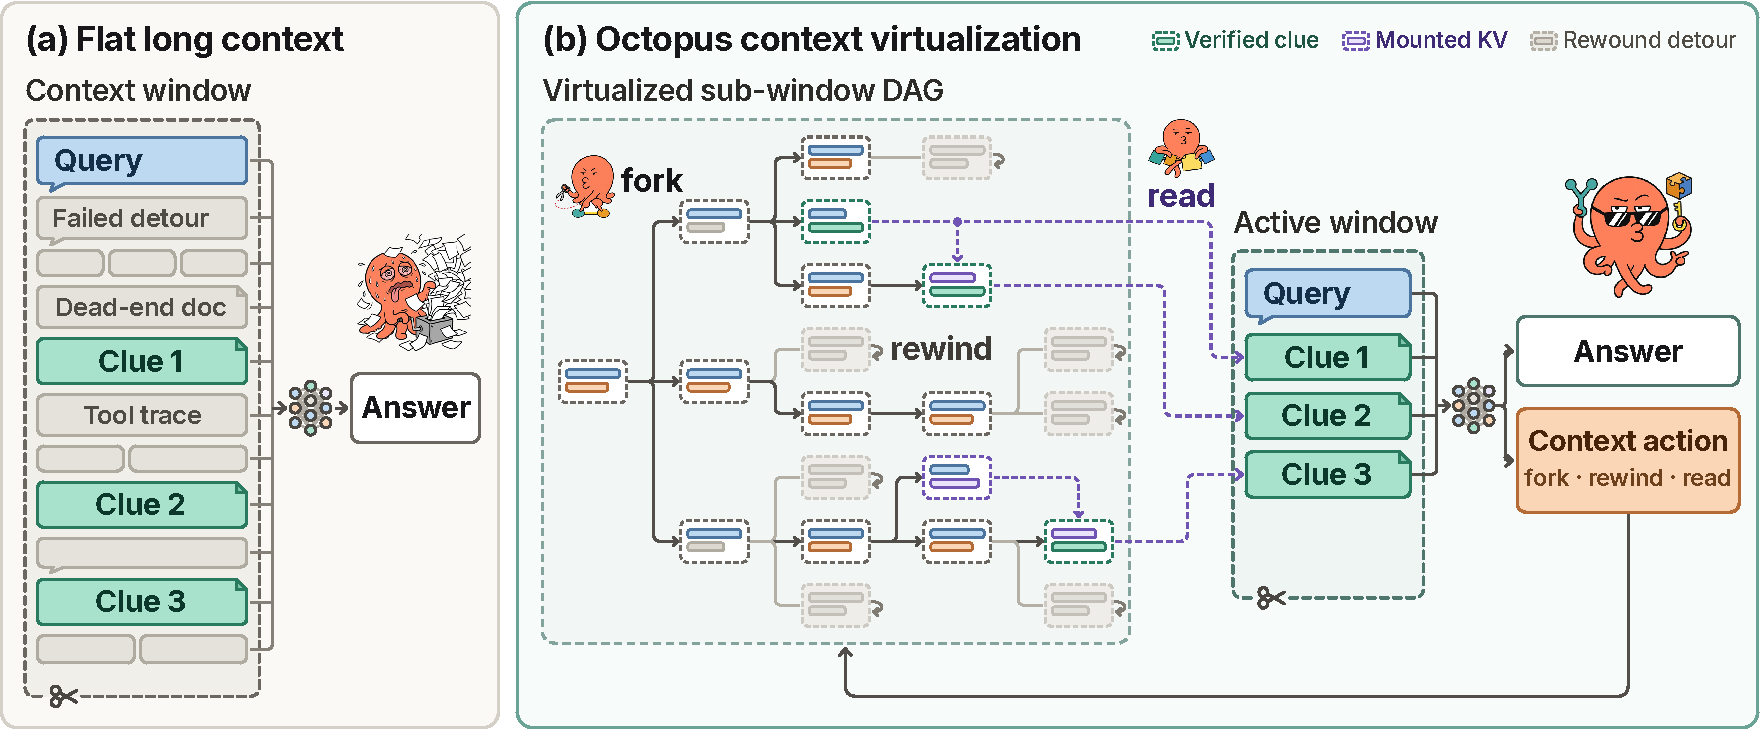
\includegraphics[width=\textwidth]{figures/fig1_overview.pdf}
\end{minipage}
\clearpage

\section{Introduction}
\label{sec:intro}

Deep search and multi-hop reasoning are inherently branching processes: an agent decomposes a question into parallel sub-queries, abandons dead-end detours, cross-checks sibling findings, and synthesizes verified evidence \citep{jin2025searchr1, chen2025browsecompplus, li2026openresearcher}. Yet modern serving engines, agent harnesses, and reinforcement learning (RL) trainers execute every episode as a flat, append-only text sequence \citep{yao2023react, wu2023autogen, hong2023metagpt, wang2025ragen, fu2025areal}. Forcing tree-structured exploration onto a single linear context creates an immediate trilemma. A standard $32\text{K}$ window saturates after opening just a few $8\text{K}$-token web pages, capping a $4\text{B}$ agent at $26.0\%$ accuracy on BrowseComp-Plus (\cref{tab:main-search}). Stretching that flat window to $143\text{K}$ under RL lifts accuracy to only $32.1\%$ and stalls at $28.5\%$ capacity ($40.8\text{K}$ tokens), because failed detours remain in working memory and dilute attention over true evidence \citep{liu2024lost, fu2026akv}. Meanwhile, compacting or editing prior turns in place \citep{cassano2026cursor, wu2025resum, zhou2026mem1, li2026acm, shao2026clm} discards exact identifiers, breaks append-only prefix KV caching, and invalidates sequential recurrent states in modern hybrid architectures such as Gated DeltaNet \citep{yang2024gated} and Mamba-2 \citep{dao2024transformers}.

Breaking out of a single flat window requires native branching execution, yet existing multi-agent, KV-sharing, and RL systems hit three structural walls. First, client-side multi-agent harnesses coordinate workers over stateless chat APIs, re-transmitting text histories and duplicating shared prefixes across sessions \citep{li2023camel, wu2023autogen, hong2023metagpt, khatua2026cooperbench}. Second, inference-time KV-sharing methods splice or re-rotate caches across all layers indiscriminately \citep{yao2025cacheblend, rodionov2025hogwild, ye2025kvcomm, jeon2026kvcmas}; in hybrid recurrent-attention models, stepping recurrent states through a sibling's text or full-layer cache overwrites the reader's sequential working memory and hijacks over half of subsequent turns ($55.2\%$--$57.9\%$; \cref{tab:kv-probe}). Third, existing branching RL frameworks exchange findings only as re-encoded text summaries \citep{pan2025apr, sun2025contextfolding, hong2025mgrpo}, while naive sequence-level tree training either overcounts shared prefixes or severs cross-branch KV dependencies.

We introduce \textbf{Octopus} (\cref{fig:overview}), a co-designed serving runtime, GPU memory manager, and RL framework that replaces the flat text tape with a GPU-resident execution DAG. Agents coordinate directly over immutable server-side radix cursors through five primitives: \texttt{fork} shares the parent's KV prefix in $\mathcal{O}(1)$ while granting each child a clean $32\text{K}$ growth budget; \texttt{rewind} rolls back dead-end detours and restores hybrid recurrent checkpoints $\mathbf{h}_k$; \texttt{read\_thread} mounts sibling KV pages in zero copy; and \texttt{wait} and \texttt{done} synchronize results. Two co-designed mechanisms make latent cross-branch execution both hijack-free and end-to-end trainable. First, Octopus decouples sequential working memory from associative recall in hybrid models \citep{afendulev2026attention}: \texttt{read\_thread} splices sibling KV pages exclusively into full-attention layers under a monotonic position offset, while recurrent layers skip mounted spans. This zero-copy mount allocates zero new KV pages, retains $92.2\%$ of full-text answer information, and cuts off-task hijacking by $21\times$ ($57.9\% \to 2.7\%$). Second, our 1D packed DAG kernel and \textbf{DAG-GRPO} objective deduplicate shared prefixes via single-ownership masking while keeping mounted KV edges live in the forward--backward graph. Retaining live mount edges cuts rollout--training divergence by $32\times$ ($\mathrm{KL} = 0.0142 \to 4.45 \times 10^{-4}$) and routes reader gradients directly into producer KV projections, keeping cross-branch latent communication strictly on-policy and end-to-end differentiable.

Trained on Qwen3.5-4B using pure binary outcome rewards with zero process shaping \citep{deepseek2025r1}, Octopus discovers a self-organized division of labor from scratch (\cref{fig:topology-dynamics}). Without RL, exposing branching primitives yields no gain over $32\text{K}$ single-agent ReAct ($26.3\%$ vs.\ $26.0\%$). Under DAG-GRPO, the policy undergoes a sharp phase transition at Step~$15$: the root thread evolves into a dedicated commander that forks on Turn~$1$ in $98.0\%$ of episodes (up $38\times$), offloads $92.8\%$ of $8\text{K}$-page reads and $91.5\%$ of rewinds to sub-agents, and coordinates a peer-to-peer latent KV mesh averaging $23.9$ zero-copy mounts per episode. Disabling \texttt{fork} at test time on the exact same trained weights collapses paired BrowseComp-Plus accuracy by $21.7$ points ($50.8\% \to 29.1\%$), proving that gains come from live collective execution rather than weight memorization.

Isolating noisy document reads across clean $32\text{K}$ branches keeps per-turn active prompts at $26.4\text{K}$ tokens while scaling explored context to $329.2\text{K}$ ($199.0\text{K}$ net surviving), compressing critical-path length by $1.94\times$, more than doubling gold-document opening recall ($21.1\% \to 43.3\%$), and lifting accuracy on the hardest multi-hop queries by $10\times$ ($3.4\% \to 34.1\%$). Overall, Octopus-$4\text{B}$ under sparse BM25 reaches $51.2\%$ on OpenResearcher and $49.6\%$ on BrowseComp-Plus ($+17.5$ points over $143\text{K}$ Single-Agent GRPO; \cref{fig:search-pareto}, \cref{tab:main-search}). Despite its $4\text{B}$ footprint, Octopus surpasses $9\text{B}$ context-editing RL ($42.5\%$) \citep{shao2026clm}, matches snippet-only OpenAI o3 under BM25 ($49.3\%$), and outperforms dense-retrieval browser agents up to $250\times$ larger---including $30\text{B}$ Tongyi-DeepResearch ($44.5\%$), $671\text{B}$ DeepSeek-R1 ($16.4\%$), $1\text{T}$ Kimi-K2 ($35.4\%$), GPT-4.1 ($36.4\%$), and Claude~4 Opus ($36.8\%$). Our contributions are:
\begin{enumerate}[leftmargin=15pt, itemsep=1.2pt, topsep=1.5pt, parsep=0pt]
  \item \textbf{GPU-Native Branching Execution Primitives (\cref{sec:method-framework,sec:exp-scalability}):} We formulate long-horizon exploration as a GPU-resident execution DAG over five primitives (\texttt{fork}, \texttt{rewind}, \texttt{read\_thread}, \texttt{wait}, and \texttt{done}) with isolated $32\text{K}$ branch budgets and bounded runtime admission.
  \item \textbf{Hijack-Free Zero-Copy KV Mounting (\cref{sec:method-cursor-mount,sec:exp-efficiency}):} We splice sibling KV pages exclusively into full-attention layers under monotonic position offsets while recurrent layers skip mounted spans, retaining $92.2\%$ answer information and cutting hijacking $21\times$ ($57.9\% \to 2.7\%$).
  \item \textbf{Server-Resident Radix Cursors and 1D Packed DAG Kernels (\cref{sec:method-kernels,sec:exp-efficiency}):} We bind turns to immutable GPU radix cursors ($89.6\%$ KV cache hit rate) and compile prefix trees, recurrent checkpoints, and KV mounts into one 1D forward--backward pass.
  \item \textbf{Latent-Communication Tree RL and Emergent Collective Scaling (\cref{sec:method-dag-grpo,sec:exp-main,sec:exp-scalability}):} We introduce DAG-GRPO with single-ownership masking and live mount edges ($32\times$ lower rollout--training KL), eliciting emergent multi-agent division of labor and lifting Qwen3.5-4B to $49.6\%$ on BrowseComp-Plus and $51.2\%$ on OpenResearcher.
\end{enumerate}

\vspace{-4pt}
\section{Related Work}
\label{sec:related}
\vspace{-2pt}

\paragraph{Active Context Management, Compaction, and Branch-and-Return Folding.}
To operate within finite context budgets, recent agent harnesses periodically summarize history \citep{cassano2026cursor, wu2025resum}, consolidate memory every turn \citep{zhou2026mem1, wu2026activemem}, or expose explicit compression and offloading tools \citep{li2026selfcompact, li2026acm, li2026sculptor, zhang2025rlm, kontonis2026memento}. Context Language Models (CLM) paired with Suffix Cache Reuse (SCR) \citep{shao2026clm} allow in-place context edits, but mid-context mutations break prefix caching, force suffix copy and RoPE re-rotation, and invalidate sequential recurrent states in hybrid models. Closer to our setting, Context-Folding \citep{sun2025contextfolding} folds sub-trajectories sequentially at depth~$1$, while Adaptive Parallel Reasoning (APR) \citep{pan2025apr} spawns parallel child threads under RL. However, both return compressed text summaries upon joining a branch---discarding exact identifiers and preventing lateral peer reads---and neither snapshots or rolls back hybrid recurrent states (\cref{tab:related-comparison}). Octopus instead executes concurrent, unlimited-depth trees over shared GPU radix prefixes, supports exact recurrent-state backtracking, and shares sibling findings directly via zero-copy attention KV mounting.

\paragraph{Multi-Agent Harnesses and Cross-Agent KV Sharing.}
Existing multi-agent harnesses \citep{li2023camel, wu2023autogen, hong2023metagpt, khatua2026cooperbench} coordinate workers above stateless chat APIs, incurring repeated prompt re-transmission, re-tokenization, and quadratic KV duplication across sessions. To bypass text serialization, inference-time KV-sharing methods select attention layers in pure Transformers \citep{shi2025kvcomm} or splice and RoPE-rerotate KV blocks across contexts \citep{gim2024promptcache, yao2025cacheblend, hu2025epic, liu2024droidspeak, rodionov2025hogwild, ye2025kvcomm, jeon2026kvcmas}, while Cache-to-Cache \citep{fu2026c2c} and DiffMAS \citep{yu2026diffmas} train supervised KV fusion modules on fixed graphs. Yet none of these methods support dynamic branching trees under on-policy RL, prevent recurrent-state corruption in hybrid architectures \citep{dao2024transformers, yang2024gated, afendulev2026attention}, or avoid RoPE phase inversion when a sibling branch runs longer than the reader. Octopus resolves all three limitations by splicing sibling KV pages exclusively into full-attention layers under rotation-free monotonic position offsets while recurrent layers skip mounted spans.

\paragraph{Reinforcement Learning for Long-Horizon and Branching Agents.}
Multi-turn agentic RL \citep{jin2025searchr1, wang2025ragen, fu2025areal, zhang2026arealdta, wang2026qwengyre, sun2026multiagentopd} and stepwise context-editing RL \citep{wu2025resum, li2026sculptor, shao2026clm} optimize flat trajectories segmented at turn or edit boundaries. Existing branching and hierarchical RL methods \citep{pan2025apr, sun2025contextfolding, hong2025mgrpo} exchange findings across branches only as re-encoded text summaries, whereas flattening trees into disconnected sequences either overcounts shared prefixes or drops cross-branch KV mounts. Octopus instead compiles prefix trees, recurrent-state rewinds, and live KV mount edges into one on-policy training graph ($\mathrm{KL} = 4.45\times 10^{-4}$ vs.\ $0.0142$ without mounts; \cref{sec:exp-scalability}), routing reader gradients directly into producer KV projections. To our knowledge, Octopus is the first on-policy RL system for agents that communicate through shared latent KV states, and the first on hybrid recurrent-attention models.

\begin{table}[!htb]
\centering
\caption{Six-dimension architectural comparison between \textbf{Octopus} and five existing long-horizon agent paradigms (\cmarkyes~supported, \cmarkpart~partial / degraded, \cmarkno~unsupported / vulnerable).}
\label{tab:related-comparison}
\setlength{\tabcolsep}{4.2pt}
\setlength{\aboverulesep}{0pt}
\setlength{\belowrulesep}{0pt}
\renewcommand{\arraystretch}{1.08}
\resizebox{\textwidth}{!}{%
\begin{tabular}{lcccccc}
\toprule
\rowcolor{hdrbg}
\lcell{\textbf{System, Memory}\\\textbf{\& RL Dimension}} &
\mcell{\textbf{1.\ Long Window}\\(Qwen-1M /\\Single-Agent RL)} &
\mcell{\textbf{2.\ Edit / Fold}\\(CLM+SCR /\\Context-Folding)} &
\mcell{\textbf{3.\ Multi-Agent}\\(AutoGen /\\CAMEL / APR)} &
\mcell{\textbf{4.\ Prior KV Sharing}\\(Blend / Hogwild! /\\KVComm)} &
\mcell{\textbf{5.\ Sequence Agent RL}\\(Search-R1 / RAGEN\\+ Leaf-Split Trees)} &
\cellcolor{oursrow}\octorelated{octo_21_title_boss}\mcell{{\color{ourstext}\textbf{Octopus (Ours)}}\\(Cursor + Attn Mount\\+ DAG-GRPO)} \\
\midrule
\octorelated{octo_fork}\lcell{\textbf{1.\ Execution}\\\textbf{Topology \&}\\\textbf{Isolation}} &
\mcell{\cmarkno~\textbf{Flat Linear}\\Detour pollution\\dilutes attention} &
\mcell{\cmarkpart~\textbf{Sequential Fold}\\Depth-$1$ serial;\\no path speedup} &
\mcell{\cmarkyes~\textbf{Parallel Chats}\\Isolated sessions,\\no shared KV} &
\mcell{\cmarkyes~\textbf{Parallel Tree}\\Inference-only\\KV block sharing} &
\mcell{\cmarkno~\textbf{Flat Sequences}\\Single-chain rollout\\or leaf-split tree} &
\cellcolor{oursrow}\mcell{\cmarkyes~{\color{ourstext}\textbf{Parallel CoW Tree + DAG}}\\Unlimited depth ($32\text{K}$/branch)\\+ lateral peer \texttt{read}} \\
\midrule
\octorelated{octo_08_chat_retok}\lcell{\textbf{2.\ Per-Turn}\\\textbf{Wire \& Token}\\\textbf{Protocol}} &
\mcell{\cmarkno~\textbf{$\mathcal{O}(L)$ Resend}\\Full history resend\\\& template drift} &
\mcell{\cmarkno~\textbf{Re-Tokenize}\\Re-renders prompt\\after mid-edits} &
\mcell{\cmarkno~\textbf{$\mathcal{O}(NL)$ Resend}\\Repeated text\\serialization} &
\mcell{\cmarkpart~\textbf{Block Sync}\\External position\\\& block tracker} &
\mcell{\cmarkno~\textbf{$\mathcal{O}(L)$ Stitch}\\Re-tokenizes flat\\turns every step} &
\cellcolor{oursrow}\mcell{\cmarkyes~{\color{ourstext}\textbf{$\mathcal{O}(\Delta)$ Server Cursor}}\\Immutable radix cursor\\+ startup template probe} \\
\midrule
\octorelated{octo_radix}\lcell{\textbf{3.\ Prefix KV}\\\textbf{\& Hybrid}\\\textbf{State Reuse}} &
\mcell{\cmarkpart~\textbf{Append-Only}\\Invalidated upon\\any backtrack} &
\mcell{\cmarkno~\textbf{Breaks Recurrence}\\Mid-edit / fold\\invalidates state} &
\mcell{\cmarkno~\textbf{$\mathcal{O}(N^2)$ Isolated}\\$0\%$ cross-agent\\KV cache reuse} &
\mcell{\cmarkno~\textbf{Attn-Only / All-Layer}\\Corrupts hybrid\\recurrent state} &
\mcell{\cmarkno~\textbf{Recomputes $K\times$}\\Repeats shared\\trunk per leaf} &
\cellcolor{oursrow}\mcell{\cmarkyes~{\color{ourstext}\textbf{Shared GPU Radix Tree}}\\\textbf{$\mathcal{O}(1)$} ref-counted KV prefix\\+ cloned recurrent state} \\
\midrule
\octorelated{octo_10_layer2_mount}\lcell{\textbf{4.\ Cross-Branch}\\\textbf{KV Sharing \&}\\\textbf{Hijack Safety}} &
\mcell{\textbf{---}\\Single-thread\\execution only} &
\mcell{\cmarkno~\textbf{Lossy Text Return}\\Drops IDs; text\\pollutes memory} &
\mcell{\cmarkno~\textbf{$+L$ Text Copy}\\Raw transcript\\hijacks reader} &
\mcell{\cmarkno~\textbf{$+L$ Copy / Unshifted}\\RoPE copy pages or\\longer-sibling flip} &
\mcell{\textbf{---}\\No cross-branch\\state reading} &
\cellcolor{oursrow}\mcell{\cmarkyes~{\color{ourstext}\textbf{$0$-Copy Attn KV Mount}}\\Recurrent layers skip mount\\+ monotonic pos.\ offset} \\
\midrule
\octorelated{octo_20_commit_gate}\lcell{\textbf{5.\ Backtrack}\\\textbf{Recovery \&}\\\textbf{Tree Closure}} &
\mcell{\cmarkno~\textbf{No Backtrack}\\Dead-end docs\\remain in window} &
\mcell{\cmarkpart~\textbf{KV Truncate Only}\\No recurrent snap\\or lateral \texttt{read}} &
\mcell{\cmarkno~\textbf{No State Rewind}\\Cannot roll back\\branch KV or state} &
\mcell{\cmarkno~\textbf{No State Snap}\\Cannot roll back\\recurrent state} &
\mcell{\cmarkno~\textbf{No Branch Rewind}\\Append-only turn\\rollout buffer} &
\cellcolor{oursrow}\mcell{\cmarkyes~{\color{ourstext}\textbf{Exact State Checkpoint}}\\Reclaims branch budget\\+ verified close contract} \\
\midrule
\octorelated{octo_dag}\lcell{\textbf{6.\ RL Kernel}\\\textbf{\& Rollout}\\\textbf{Alignment}} &
\mcell{\cmarkno~\textbf{Detour Noise}\\Failed detours\\dilute credit} &
\mcell{\cmarkpart~\textbf{Cut at Segments}\\No cross-branch\\KV mount edges} &
\mcell{\cmarkno~\textbf{No Shared-KV RL}\\Independent chats or\\text-summary joins} &
\mcell{\cmarkno~\textbf{Inference-Only}\\No packed tree\\training kernel} &
\mcell{\cmarkno~\textbf{Drops KV Mounts}\\Sequence pass breaks\\rollout alignment} &
\cellcolor{oursrow}\mcell{\cmarkyes~{\color{ourstext}\textbf{1D Packed DAG Kernel}}\\Single-ownership loss mask\\+ live on-policy mounts} \\
\bottomrule
\end{tabular}%
}
\end{table}
\renewcommand{\best}[1]{{\color{ourstext}\bfseries #1}}
\renewcommand{\bad}[1]{{\color{badtext}\bfseries #1}}

\section{Method}
\label{sec:method}

Instead of re-sending growing chat transcripts on every turn, Octopus models a long-horizon episode as a cursor-addressed execution DAG $\mathcal{G} = (\mathcal{V}, \mathcal{E}_{\text{tree}}, \mathcal{E}_{\text{mount}})$. Analogous to an OS copy-on-write handle, each vertex $c \in \mathcal{V}$ is a lightweight cursor ID referencing an immutable snapshot of physical KV pages and recurrent state resident in GPU memory. Directed tree edges $(c \to c') \in \mathcal{E}_{\text{tree}}$ capture vertical state transitions (turn continuation, parallel \texttt{fork}, and \texttt{rewind}), whereas directed mount edges $(c_A \leadsto c_B) \in \mathcal{E}_{\text{mount}}$ capture horizontal coordination (\texttt{read\_thread}), allowing branch $B$ to attend directly to sibling $A$'s physical KV pages. Octopus co-designs four layers around $\mathcal{G}$ (\cref{fig:overview}): branching execution primitives (\cref{sec:method-framework}), layer-selective monotonic KV mounting (\cref{sec:method-cursor-mount}), server-resident radix cursors and 1D packed DAG kernels (\cref{sec:method-kernels}), and on-policy DAG-GRPO training (\cref{sec:method-dag-grpo}).

\subsection{Branching Execution Primitives and Per-Branch Isolation}
\label{sec:method-framework}

\begin{figure}[!t]
\centering
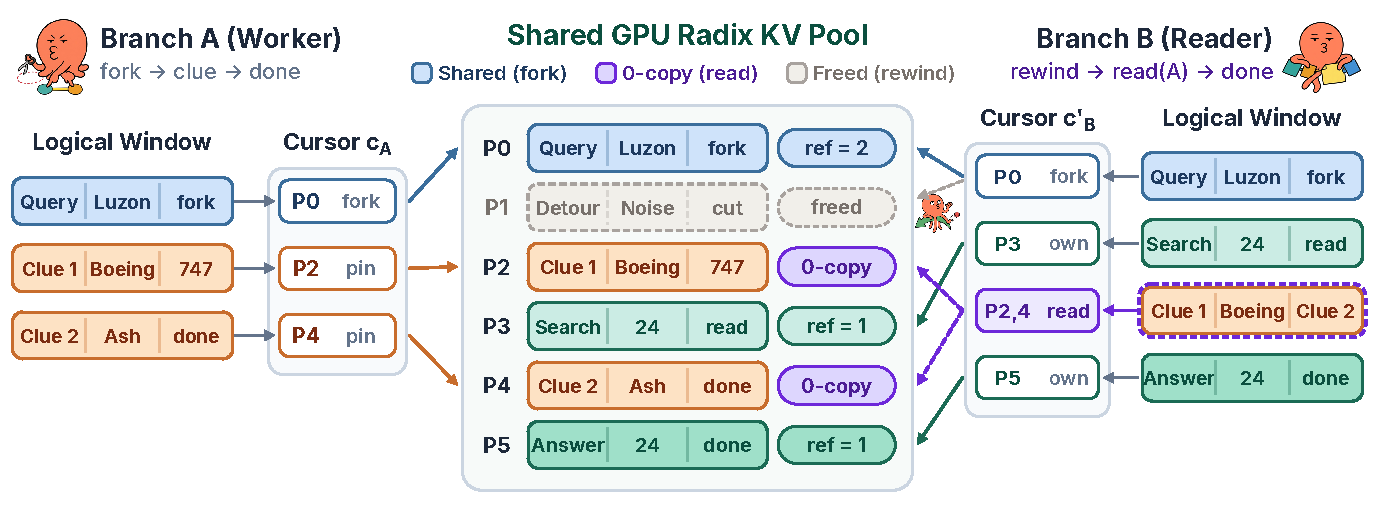
\includegraphics[width=1.0\textwidth]{figures/fig_sec31_paged.pdf}
\caption{Cursor-addressed page translation and zero-copy KV page lending in Octopus (\cref{sec:method-framework,sec:method-kernels}). Worker and reader branches maintain isolated logical windows backed by a shared GPU radix KV pool: \texttt{fork} shares the parent prefix in $\mathcal{O}(1)$ (\texttt{ref\,=\,2}), \texttt{rewind} reclaims dead-end pages, and \texttt{read} mounts pinned sibling KV pages in zero copy without allocating new physical blocks.}
\label{fig:paged-cursor}
\end{figure}

Existing single- and multi-agent harnesses sit above the serving engine, either enforcing a flat append-only loop or stitching stateless chat sessions at $\mathcal{O}(L)$ wire cost and $\mathcal{O}(N^2)$ KV duplication. Octopus instead co-designs the multi-agent harness with the GPU memory manager, running branches as lightweight GPU-resident threads across five primitives with isolated budgets and explicit closing contracts (\cref{fig:paged-cursor}, \cref{tab:primitives}).

\begin{table}[!htb]
\centering
\caption{Summary of the five execution primitives in Octopus (\cref{sec:method-framework}), their server-side cursor and KV-cache semantics, and their control-flow and budget semantics.}
\label{tab:primitives}
\footnotesize
\setlength{\tabcolsep}{4.2pt}
\setlength{\aboverulesep}{0pt}
\setlength{\belowrulesep}{0pt}
\renewcommand{\arraystretch}{1.04}
\newcommand{\pbox}[2]{\rule[-4.55ex]{0pt}{9.65ex}\parbox[c]{#1}{\raggedright\setlength{\baselineskip}{9.8pt}#2}}
\resizebox{\textwidth}{!}{%
\begin{tabular}{l l c c}
\toprule
\rowcolor{hdrbg}
\multicolumn{1}{c}{\rowstrut\textbf{Primitive}} & \multicolumn{1}{c}{\textbf{Signature}} & \multicolumn{1}{c}{\textbf{Cursor \& KV-Cache Semantics}} & \multicolumn{1}{c}{\textbf{Control-Flow \& Budget Semantics}} \\
\midrule
\rowcolor{oursrow}
\rule[-4.55ex]{0pt}{9.65ex}\octotabone{octo_fork}\textbf{\texttt{fork}} & \pbox{3.32cm}{\texttt{fork(branches=\\\{id:\ prompt\})}} & \pbox{4.95cm}{Clones parent cursor node in $\mathcal{O}(1)$; shares radix KV prefix; clones recurrent state $\mathbf{h}_{\text{end}}(c_{\text{fork}})$.} & \pbox{5.25cm}{Spawns parallel child branches, each granted a fresh $B_{\text{thread}} = 32\text{K}$ token growth budget.} \\
\rule[-4.55ex]{0pt}{9.65ex}\octotabone{octo_radix}\textbf{\texttt{read}} & \pbox{3.32cm}{\texttt{read(branch,\\steps=[a, b])}} & \pbox{4.95cm}{Zero-copy lends branch $A$'s KV pages to attention layers $\mathcal{L}_{\text{mount}}$ w/ monotonic pos.\ (\cref{eq:k2-pos}); recurrent layers skip span.} & \pbox{5.25cm}{Injects a compact metadata stub ($\sim 15$ tokens) into reader $B$'s prompt without copying $A$'s text.} \\
\rowcolor{oursrow}
\rule[-4.55ex]{0pt}{9.65ex}\octotabone{octo_19_wait_sleep}\textbf{\texttt{wait}} & \pbox{3.32cm}{\texttt{wait(branches=[...])}} & \pbox{4.95cm}{Suspends caller cursor until target child branches reach terminal \texttt{COMPLETED} state.} & \pbox{5.25cm}{Returns brief branch status summaries and step manifests available for \texttt{read}.} \\
\rule[-4.55ex]{0pt}{9.65ex}\octotabone{octo_17_rewind_cut}\textbf{\texttt{rewind}} & \pbox{3.32cm}{\texttt{rewind(step=k,\\note)}} & \pbox{4.95cm}{Restores cursor $c_k$ and exact recurrent state snapshot $\mathbf{h}_k$ at step $k$; appends diagnostic \texttt{note}.} & \pbox{5.25cm}{Reclaims dead-end token budget ($k+1\dots t$) while retaining the pruned branch in the training DAG.} \\
\rowcolor{oursrow}
\rule[-4.55ex]{0pt}{9.65ex}\octotabone{octo_20_commit_gate}\textbf{\texttt{done}} & \pbox{3.32cm}{\texttt{done(answer,\\evidence)}} & \pbox{4.95cm}{Marks branch or root cursor \texttt{COMPLETED} and pins its KV pages in GPU radix pool for parent/sibling \texttt{read}.} & \pbox{5.25cm}{Enforced by a $2\text{K}$ answer reserve and $1$-turn close reminder; returns verified answer and evidence.} \\
\bottomrule
\end{tabular}%
}
\end{table}

\paragraph{Orchestrator--Worker Coordination.}
An episode begins at a root orchestrator thread and expands recursively into concurrent worker branches. Calling \texttt{fork} at cursor $c_{\text{fork}}$ spawns $K$ parallel children in $\mathcal{O}(1)$ zero copy: all children share the parent's GPU KV prefix pages via reference counting ($+K$) while each receives a cloned recurrent state $\mathbf{h}_{\text{end}}(c_{\text{fork}})$. When a search query or $8\text{K}$-token page open hits a dead end, \texttt{rewind} rolls the cursor back to step $k$, restores the exact recurrent checkpoint $\mathbf{h}_k$, reclaims steps $k+1 \dots t$ from the branch budget, and appends a short diagnostic \texttt{note}. For horizontal sharing, \texttt{read\_thread} (abbreviated \texttt{read} in \cref{tab:primitives}) mounts a completed step range $[a, b]$ from a sibling or cousin branch directly into the caller's full-attention layers without copying text or advancing recurrent states. Parents synchronize via \texttt{wait}, and every thread closes via \texttt{done}.

\paragraph{Per-Branch Budgets and Runtime Guardrails.}
Each thread operates under an independent growth budget $B_{\text{thread}} = 32{,}768$ tokens (with $R_{\text{ans}} = 2{,}048$ tokens reserved for final synthesis): only newly appended or generated tokens consume $B_{\text{thread}}$, whereas inherited parent prefixes and mounted sibling KV pages are shared in zero copy. To preserve prefix KV caching and prevent server saturation or unclosed rollouts, Octopus injects the \texttt{read\_thread} tool card append-only once a peer step becomes readable, gates new episode admission when GPU KV pool usage exceeds $\tau_{\text{KV}} = 0.75$, and issues a single-turn untrainable reminder if a thread emits plain text instead of \texttt{done} (Appendix~\ref{app:runtime-details}).

\subsection{Layer-Selective Monotonic KV Mounting}
\label{sec:method-cursor-mount}

\begin{figure}[!t]
\centering
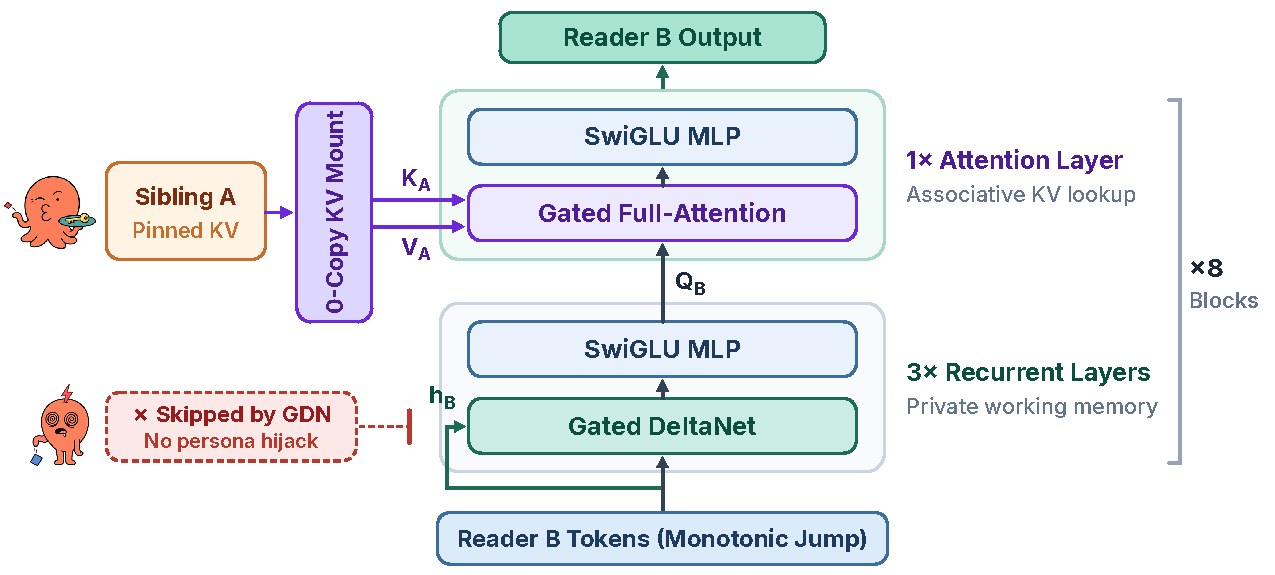
\includegraphics[width=0.92\textwidth]{figures/fig_sec32_yoco.pdf}
\caption{Layer-selective cross-branch KV mounting in hybrid recurrent-attention blocks (\cref{sec:method-cursor-mount}). Pinned sibling KV pages ($K_A, V_A$) are spliced in zero copy exclusively into full-attention layers for associative lookup, while recurrent Gated DeltaNet layers advance only the reader's private working memory $\mathbf{h}_B$ over post-mount tokens to prevent persona hijacking.}
\label{fig:cursor-mount}
\end{figure}

Sharing sibling findings via raw text injection or all-layer KV splicing causes reader branch $B$ to abandon its own goal and pursue sibling $A$'s task in over half of interactions (\cref{sec:exp-mechanism}). We resolve this conflict by exploiting how recurrent and full-attention layers physically store history (\cref{fig:cursor-mount}).

\paragraph{Decoupling Recurrent Working Memory from Associative Attention Lookup.}
Modern long-context backbones interleave linear recurrent layers (e.g., Gated DeltaNet or Mamba-2) with sparse full-attention layers \citep{dao2024transformers, yang2024gated}. Crucially, a recurrent layer compresses history into a fixed-size rolling state $\mathbf{h}_B$ that is mutated by every incoming token, whereas a full-attention layer stores KV pages passively and reads them only when queried \citep{afendulev2026attention} (in pure-attention models, a sparse subset of middle retrieval layers plays an analogous role; Appendix~\ref{app:arch-blueprints}). Feeding sibling $A$'s trajectory through recurrent layers directly overwrites $\mathbf{h}_B$---replacing $B$'s active persona and goal with $A$'s---whereas mounting $A$'s KV pages into target full-attention layers $\mathcal{L}_{\text{mount}} \subseteq \mathcal{L}_{\text{attn}}$ exposes $A$'s evidence as a passive lookup table. When reader $B$ (at cursor $c_B$) mounts span $[s_A, e_A)$ from $c_A$, Octopus splices $c_A[s_A : e_A)$ exclusively into $\mathcal{L}_{\text{mount}}$ and skips $[s_A, e_A)$ in all recurrent layers, advancing $\mathbf{h}_B$ solely over $B$'s post-mount tokens $\Delta_B$ from $\mathbf{h}_{\text{end}}(c_B)$. Retrieved attention features on $\Delta_B$ still inform deeper recurrent layers ($l > l_{\text{attn}}$) via residuals without $A$'s raw tokens overwriting $\mathbf{h}_B$.

\paragraph{Rotation-Free Monotonic Position Continuation.}
Splicing foreign KV pages into full-attention layers creates relative-position conflicts under 1D/M-RoPE (\cref{fig:rope-streaming}), where attention scores depend on query--key phase differences:
\begin{equation}
\label{eq:rope-phase}
\langle \mathcal{R}_{q}\mathbf{q},\, \mathcal{R}_{k}\mathbf{k} \rangle = \mathrm{Re}\!\left(\sum_{d} q_d k_d^* \, e^{i(q - k)\theta_d}\right).
\end{equation}
Let $p_B = \mathrm{pos}_{\text{next}}(c_B)$ denote $B$'s next unshifted position. Whenever sibling $A$ has progressed further in token index than $B$ ($e_A > p_B$), leaving $B$'s queries at $q_B = p_B$ yields negative relative distances $q_B - k_A < 0$ for mounted keys $k_A \in (p_B, e_A)$, placing $A$'s keys in $B$'s causal future with inverted RoPE phases. Conversely, copying and RoPE-rerotating $A$'s keys into $B$'s local frame \citep{rodionov2025hogwild, shi2025kvcomm, ye2025kvcomm} duplicates GPU memory per reader. Octopus instead keeps mounted KV pages at their native positions and jumps $B$'s post-mount tokens $\Delta_B$ monotonically past the highest mounted index:
\begin{equation}
\label{eq:k2-pos}
s(c_B') = \max\!\Big(\mathrm{pos}_{\text{next}}(c_B),\; \max_{m \in \mathrm{Mounts}(c_B')} \big(\mathrm{pos}_{\text{end}}(m) + 1\big)\Big).
\end{equation}
For example, if $B$ is at position $2{,}000$ and mounts $A$'s tokens $1{,}500\text{--}4{,}000$, $B$'s next token jumps to $4{,}001$: every visible key now lies strictly in $B$'s past ($q_B - k \ge 1$) with zero KV copying, while position-free recurrent and convolution layers are unaffected. Although mounted indices $1{,}500\text{--}1{,}999$ overlap with $B$'s pre-mount tokens counted from the fork point, content-based attention keys disambiguate colliding positions without re-rotation (\cref{sec:exp-mechanism}).

\begin{figure}[!t]
\centering
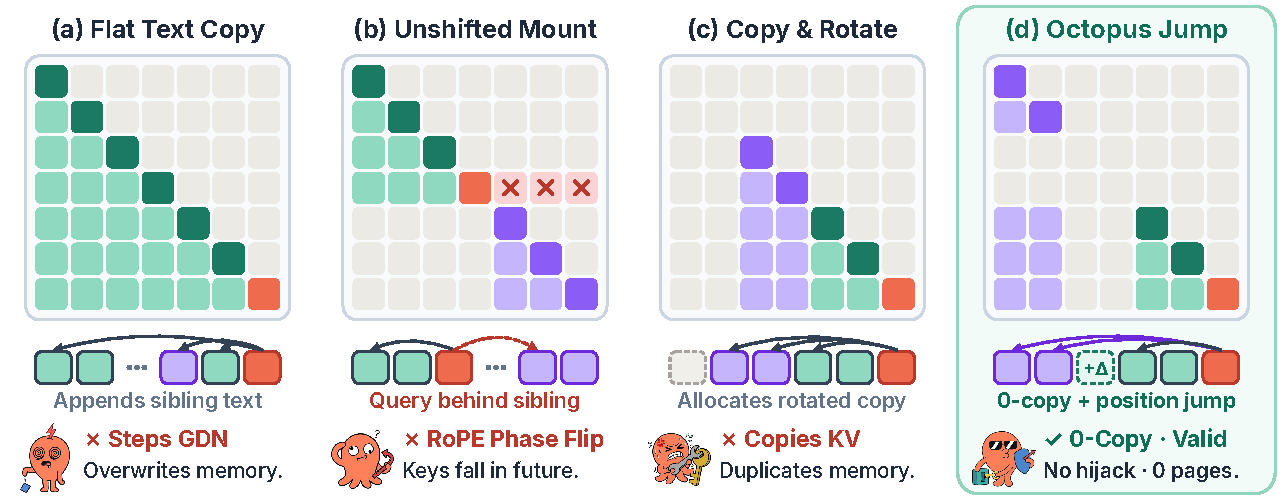
\includegraphics[width=1.0\textwidth]{figures/fig_sec33_streaming.pdf}
\caption{Comparison of cross-branch context sharing regimes (\cref{sec:method-cursor-mount,sec:method-kernels}): (a) flat text copying steps recurrent layers and causes task hijacking; (b) unshifted KV mounting inverts RoPE relative phases whenever sibling keys exceed the reader's position; (c) copying and re-rotating KV pages duplicates GPU memory per reader; (d) Octopus retains native zero-copy KV pages and jumps post-mount query positions monotonically under causal gathering.}
\label{fig:rope-streaming}
\end{figure}

\subsection{Server-Resident Radix Cursors and 1D Packed DAG Kernels}
\label{sec:method-kernels}

\paragraph{Inference Engine: Server-Resident Radix Cursors.}
To eliminate $\mathcal{O}(L)$ prompt re-transmission across turns and forks, the serving engine stores each completed turn as an immutable cursor $c$ backed by a GPU radix prefix tree of reference-counted KV pages. Any continuation, \texttt{fork} child, or \texttt{rewind} recovery passes cursor ID $c$ and incremental messages $\Delta m$, extending the sequence in $\mathcal{O}(|\Delta m|)$ time and wire bytes:
\begin{equation}
\label{eq:delta-render}
\mathbf{x}(c') = \underbrace{\big(\mathbf{x}_{\text{prompt}}(c) \;\oplus\; \mathbf{x}_{\text{out}}^{\setminus \text{stop}}(c) \;\oplus\; \tau_{\text{term}}(c)\big)}_{\text{Immutable Server-Resident Cursor } \mathbf{x}(c)} \;\oplus\; \mathrm{Render}_\Delta\!\big(\mathcal{T},\; \Delta m,\; \mathrm{ctx}(c)\big),
\end{equation}
where $\mathbf{x}_{\text{out}}^{\setminus \text{stop}}(c)$ strips trailing stop tokens and $\tau_{\text{term}}(c)$ terminates the assistant turn. Because modern reasoning chat templates $\mathcal{T}$ are often non-append-only---for instance, stripping earlier \texttt{<think>} blocks on new user turns---a one-time ($\sim 0.1\,\text{s}$) startup probe extracts an incremental template slicer $\mathrm{Render}_\Delta$ and encodes runtime notes as tool responses, achieving bit-exact tokenization ($0/18{,}344$ mismatches across seven model families; Appendix~\ref{app:runtime-details}). Mounted KV spans are pinned via per-page reference counts and transparently re-prefilled from cursor metadata if evicted.

\begin{figure}[!t]
\centering
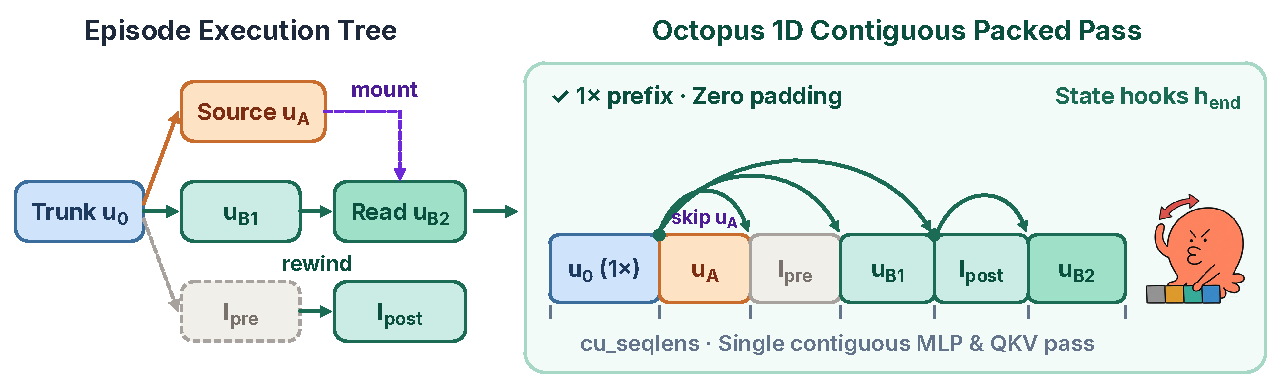
\includegraphics[width=1.0\textwidth]{figures/fig_sec33_pack.pdf}
\caption{Tree-to-1D contiguous sequence packing (\cref{sec:method-kernels}). Octopus deduplicates each tree segment once into an unpadded 1D strip and passes recurrent states $\mathbf{h}_{\text{end}}(p(u))$ across segment boundaries while skipping mounted sibling spans.}
\label{fig:dag-pack}
\end{figure}

\paragraph{Training Engine: Tree-to-1D Contiguous Packed DAG Kernels.}
Splitting a branched episode into separate leaf sequences during RL either recomputes shared trunks $K$ times or drops mounted KV spans. Octopus instead compiles each episode DAG into a single 1D packed forward--backward pass (\cref{fig:dag-pack}):
\begin{enumerate}[leftmargin=15pt, itemsep=1.5pt, topsep=2pt]
  \item \textbf{Node Splitting and Prefix Deduplication:} At every \texttt{fork}, \texttt{rewind}, or \texttt{read\_thread} boundary, Octopus partitions the episode into maximal contiguous token nodes $u = \big(p(u),\; \mathcal{M}(u),\; s(u)\big)$, recording tree parent $p(u)$, active mounted segments $\mathcal{M}(u)$ (including transitive mounts), and monotonic start position $s(u)$ (\cref{eq:k2-pos}). Each unique node $u$ is evaluated once regardless of how many branches or rewinds descend from it.
  \item \textbf{1D Contiguous MLP and Projection Pass:} Deduplicated nodes $\{u_1, \dots, u_M\}$ are concatenated topologically into one unpadded 1D tensor (up to $262\text{K}$ tokens) and run through all MLPs and QKV projections in one matrix pass.
  \item \textbf{Dual-Mechanism Graph Routing:} Across the packed 1D strip, recurrent and attention layers route activations along $\mathcal{G}$ via two complementary hooks. On recurrent layers (Gated DeltaNet and Mamba-2), boundary hooks initialize each node $u$ from its parent's terminal state $\mathbf{h}_{\text{end}}(p(u))$ (plus the last $w - 1 = 3$ causal-convolution tokens), accumulate $\partial \mathcal{L} / \partial \mathbf{h}$ back to $p(u)$ in backward, and skip $\mathcal{M}(u)$ (\cref{fig:dag-pack}). On each mounted full-attention layer $l \in \mathcal{L}_{\text{mount}}$, node $u$ gathers precomputed K/V tensors as (\cref{fig:dag-gather}):
  \begin{equation}
  \label{eq:dag-attn}
  \mathbf{K}_u^{(l)} = \Big[\, \bigoplus_{m \in \mathcal{M}(u)} \mathbf{K}_m^{(l)} \;\Big\|\; \mathbf{K}_{p(u)}^{(l)} \;\Big\|\; \mathbf{K}_{\text{self}(u)}^{(l)} \,\Big], \qquad \forall l \in \mathcal{L}_{\text{mount}}.
  \end{equation}
  Placing $\text{self}(u)$ at the rightmost tail exploits rectangular FlashAttention (\texttt{causal=True}; \cref{fig:rope-streaming}(d), \cref{fig:dag-gather}): whenever $|\mathbf{Q}_u| < |\mathbf{K}_u|$, FlashAttention aligns the causal triangle to the rightmost $|\mathbf{Q}_u|$ keys ($\text{self}(u)$) while leaving all preceding mounted and ancestor keys unmasked, avoiding custom 2D block-sparse masks and matching live SGLang rollouts to $|\Delta \log \pi_\theta| = 0.0038$.
\end{enumerate}

\begin{figure}[!t]
\centering
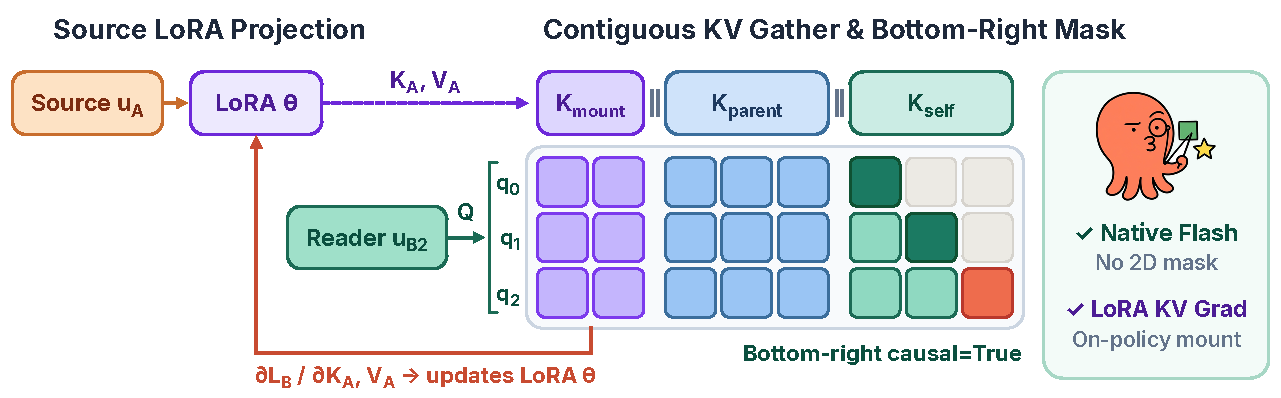
\includegraphics[width=1.0\textwidth]{figures/fig_sec33_gather.pdf}
\caption{Contiguous KV gathering and cross-branch LoRA backpropagation (\cref{sec:method-kernels,sec:method-dag-grpo}). Concatenating mounted sibling keys, ancestor prefixes, and active reader tokens places the causal diagonal at the bottom-right corner for native FlashAttention (\texttt{causal=True}), while routing $\partial \mathcal{L}_{u_B} / \partial \mathbf{K}_{u_A}, \mathbf{V}_{u_A}$ directly into source branch $A$'s LoRA adapter $\theta$.}
\label{fig:dag-gather}
\end{figure}

\subsection{DAG-GRPO Training with Single-Ownership Masking and Mounted KV Edges}
\label{sec:method-dag-grpo}

\paragraph{Single-Ownership Token Deduplication and RLOO Advantage.}
For each prompt, Octopus samples $G$ branched episode trees $\{\tau_1, \dots, \tau_G\}$ and scores each terminal outcome $y(\tau_i) \in [0, 1]$ with binary reward $R(\tau_i) = 2y(\tau_i) - 1$. Following REINFORCE Leave-One-Out (RLOO) \citep{kool2019buy}, we compute a critic-free group advantage without standard-deviation normalization (\cref{fig:dag-grpo}):
\begin{equation}
\label{eq:rloo-adv}
\hat{A}(\tau_i) = R(\tau_i) - \frac{1}{G - 1} \sum_{j \neq i} R(\tau_j),
\end{equation}
and broadcast $\hat{A}(\tau_i)$ across all threads of $\tau_i$, including rewound leaves so the \texttt{rewind} decision itself receives outcome credit. Standard sequence-RL objectives sum token losses along root-to-leaf trajectories $\{\ell \in \tau_i\}$, which on a tree naively weights each shared trunk node $u$ by its number of descendant leaves. To map trajectory-level RL directly onto our deduplicated 1D packed pass (\cref{sec:method-kernels}), we assign each node $u$ to the unique leaf $\ell = \mathrm{owner}(u)$ that first generated it via a single-ownership mask over action tokens $\mathcal{V}_{\text{gen}}(\tau_i)$:
\begin{equation}
\label{eq:single-owner-mask}
m_{\ell,t} = \mathbb{I}\Big[\ell = \mathrm{owner}(u_{\ell,t}) \;\wedge\; x_{\ell,t} \in \mathcal{V}_{\text{gen}}(\tau_i)\Big],
\end{equation}
setting $m_{\ell,t}=1$ once per generated token on the packed 1D strip and $m_{\ell,t}=0$ on prompts, tool outputs, inherited or pre-rewind prefixes ($t \le k$), and mounted sibling spans $\mathcal{M}(u)$. Summing with $m_{\ell,t}$ recovers the exact DAG score function:
\begin{equation}
\label{eq:tree-score-identity}
\sum_{\ell \in \tau_i} \sum_{t=1}^{|\ell|} m_{\ell,t} \nabla_\theta \log \pi_\theta(x_{\ell,t} \mid \mathcal{G}_{\ell,<t}) = \nabla_\theta \log \mathbb{P}_\theta(\tau_i).
\end{equation}

\begin{figure}[!htb]
\centering
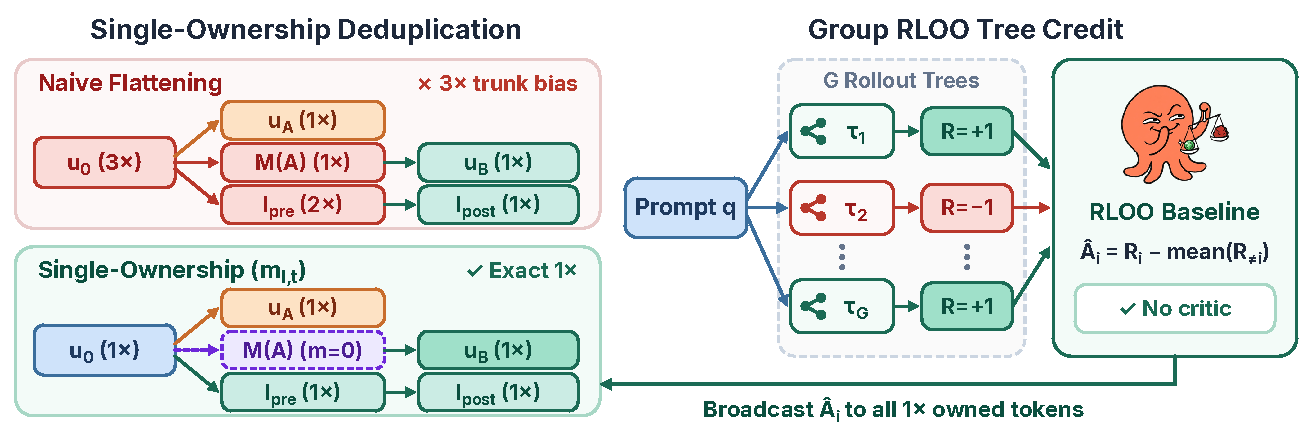
\includegraphics[width=1.0\textwidth]{figures/fig_sec34_rloo.pdf}
\caption{Single-ownership prefix deduplication and Group RLOO tree credit assignment in DAG-GRPO (\cref{sec:method-dag-grpo}). Single-ownership masking ($m_{\ell,t} \in \{0, 1\}$) counts every generated tree segment once while masking mounted spans, and broadcasts critic-free Leave-One-Out group advantages $\hat{A}(\tau_i)$ across all owned tokens.}
\label{fig:dag-grpo}
\end{figure}

\paragraph{Differentiable On-Policy Mount Edges and Clipped Objective.}
During the 1D packed pass, source node $u_A$'s keys and values at each mounted layer $l \in \mathcal{L}_{\text{mount}}$ are projected through trainable LoRA weights $\theta = \{\mathbf{B}_\theta, \mathbf{A}_\theta\}$:
\begin{equation}
\label{eq:lora-kv}
\mathbf{K}_{u_A}^{(l)}(\theta) = \big(\mathbf{W}_K^{(l)} + \mathbf{B}_{K,\theta}^{(l)} \mathbf{A}_{K,\theta}^{(l)}\big)\mathbf{H}_{u_A}^{(l)}(\theta), \qquad \mathbf{V}_{u_A}^{(l)}(\theta) = \big(\mathbf{W}_V^{(l)} + \mathbf{B}_{V,\theta}^{(l)} \mathbf{A}_{V,\theta}^{(l)}\big)\mathbf{H}_{u_A}^{(l)}(\theta),
\end{equation}
and gathered directly by reader node $u_B$ in \cref{eq:dag-attn} without detaching the mount edge. Mounted spans carry loss mask $m_{\ell,t}=0$ so $A$'s tokens are never double-counted as $B$'s actions, while attention backpropagation routes $\partial \mathcal{L}_{u_B} / \partial \mathbf{K}_{u_A}^{(l)}$ and $\partial \mathcal{L}_{u_B} / \partial \mathbf{V}_{u_A}^{(l)}$ directly into $A$'s LoRA weights (\cref{fig:dag-gather}). Unlike text-summary branching---which trains $\theta$ only on re-encoded summary tokens---keeping live mounts in the packed graph preserves on-policy rollout alignment ($\mathrm{KL} = 4.45\times 10^{-4}$ vs.\ $0.0142$ when dropped; \cref{sec:exp-systems}) and lets reader $B$'s loss directly shape how $\theta$ encodes producer $A$'s KV state. We optimize the clipped DAG-GRPO objective:
\begin{equation}
\label{eq:dag-grpo}
\mathcal{J}_{\text{DAG-GRPO}}(\theta) = \mathbb{E}_{\{\tau_i\}_{i=1}^G}\! \left[ \frac{1}{G} \sum_{i=1}^G \frac{1}{Z_i} \sum_{\ell \in \tau_i} \sum_{t=1}^{|\ell|} m_{\ell,t} \, \min\!\Big( r_{\ell,t}(\theta) \hat{A}(\tau_i),\; \mathrm{clip}\big(r_{\ell,t}(\theta), 1-\epsilon, 1+\epsilon\big) \hat{A}(\tau_i) \Big) \right],
\end{equation}
where $Z_i = \sum_{\ell \in \tau_i} \sum_{t=1}^{|\ell|} m_{\ell,t}$ counts owned generated tokens in $\tau_i$ and $r_{\ell,t}(\theta) = \pi_\theta(x_{\ell,t} \mid \mathcal{G}_{\ell,<t}) / \pi_{\theta_{\text{old}}}(x_{\ell,t} \mid \mathcal{G}_{\ell,<t})$. Normalizing by $1/Z_i$ stabilizes gradient magnitudes across trees spanning $1\text{K}$ to $199\text{K}$ tokens, though analogous to Dr.\ GRPO \citep{liu2025drgrpo} it introduces a tree-size length weighting that softens per-token penalties on failed large trees (\cref{sec:discussion}).

\section{Experiments}
\label{sec:experiments}

\begin{figure}[!htb]
\centering
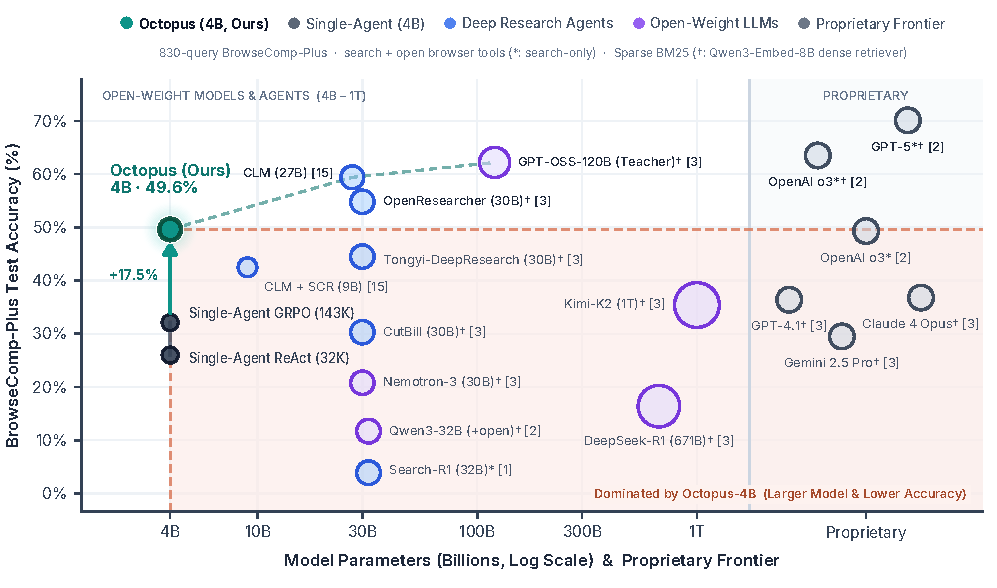
\includegraphics[width=1.0\textwidth]{figures/fig_exp1_pareto.pdf}
\caption{BrowseComp-Plus test accuracy ($830$ queries) vs.\ model parameter scale ($4\text{B}\text{--}1\text{T}$ log scale and proprietary models) \citep{chen2025browsecompplus}. Systems use browser reading tools (\texttt{search+open[+find]}) over sparse BM25 unless marked $^*$ (\texttt{search}-only) or $^\dagger$ (\texttt{Qwen3-Embed-8B} dense retrieval). \textbf{Octopus ($4\text{B}$)} reaches $\mathbf{49.6\%}$ under BM25, dominating larger open-weight and proprietary systems across the shaded region.}
\label{fig:search-pareto}
\label{fig:search-main}
\end{figure}

We evaluate Octopus around three questions:
\emph{(i) \textbf{Deep Search Performance (\cref{sec:exp-main})}}: How does a $4\text{B}$ branching agent trained with Octopus compare against proprietary frontier models, $9\text{B}$--$1\text{T}$ open-weight systems, and controlled $4\text{B}$ single-agent baselines (\cref{fig:search-pareto}, \cref{tab:main-search})?
\emph{(ii) \textbf{Context and KV-Sharing Efficiency (\cref{sec:exp-efficiency})}}: Does branch-isolated $32\text{K}$ exploration convert context into gold evidence and reuse GPU prefix caches better than flat $143\text{K}$ windows or in-place edits, and does attention-only KV mounting prevent off-task hijacking (\cref{fig:efficiency-funnel}, \cref{tab:context-conversion,tab:kv-probe})?
\emph{(iii) \textbf{Multi-Agent Scalability (\cref{sec:exp-scalability})}}: How does accuracy scale with deployed agent count and unlimited tree depth ($D_{\max}=\infty$), and what collective behaviors emerge under pure outcome RL (\cref{fig:topology-dynamics}, \cref{tab:agent-scaling})?

% ==============================================================================
% 4.1 END-TO-END DEEP SEARCH PERFORMANCE (Figure 8 + Table 3)
% ==============================================================================
\subsection{End-to-End Deep Search Performance}
\label{sec:exp-main}

\begin{table}[!t]
\centering
\caption{End-to-end deep search results on \textbf{BrowseComp-Plus} ($830$ test queries) \citep{chen2025browsecompplus} and \textbf{OpenResearcher Validation} ($500$ queries) \citep{li2026openresearcher}. Columns report prefix-reuse inference PFLOPs (\textbf{PF/Q}), accuracy under sparse BM25 ($^\dagger$dense retrieval, $^*$\texttt{search}-only), evidence recall, and critical-path vs.\ total completion tokens (\textbf{Crit.\ $C$ / Total}). \textbf{Octopus ($4\text{B}$)} lifts BrowseComp-Plus accuracy by $+17.5$ points over $143\text{K}$ Single-Agent GRPO.}
\label{tab:main-search}
\setlength{\tabcolsep}{3.5pt}
\setlength{\aboverulesep}{0pt}
\setlength{\belowrulesep}{0pt}
\renewcommand{\arraystretch}{1.13}
\resizebox{\textwidth}{!}{%
\begin{tabular}{lllcccccccc}
\toprule
\rowcolor{hdrbg}
\rowstrut & & & & \textbf{OR Val} & \multicolumn{6}{c}{\textbf{BrowseComp-Plus Official Test Benchmark (830 Queries)}} \\
\cmidrule(lr){5-5} \cmidrule(lr){6-11}
\rowcolor{hdrbg}
\hlcell{\textbf{Method /}}{\textbf{Agent System}} & \hlcell{\textbf{Backbone /}}{\textbf{Scale}} & \textbf{Tools} & \hcell{\textbf{PF/Q}}{\textbf{$\downarrow$}} & \hcell{\textbf{Val}}{\textbf{Acc.\ $\uparrow$}} & \hcell{\textbf{Test Acc.\ $\uparrow$}}{{\scriptsize\textbf{BM25 / Dense$^\dagger$}}} & \hcell{\textbf{Search}}{\textbf{Rec.\ $\uparrow$}} & \hcell{\textbf{Open}}{\textbf{Rec.\ $\uparrow$}} & \hcell{\textbf{Gold}}{\textbf{Rec.\ $\uparrow$}} & \hcell{\textbf{Context}}{\textbf{Used / Cap}} & \hcell{\textbf{Crit.\ $C$}}{\textbf{/ Total}} \\
\midrule
\rowcolor{hdrbg}
\multicolumn{11}{c}{\rowstrut{\small\textbf{Proprietary Frontier Models on BrowseComp-Plus~\citep{chen2025browsecompplus,li2026openresearcher}}}} \\
\rowstrut\textcolor{refmute}{Claude Sonnet 4~\citep{chen2025browsecompplus}} & \textcolor{refmute}{Proprietary} & \textcolor{refmute}{\texttt{s-only}$^*$} & \textcolor{refmute}{---} & \textcolor{refmute}{---} & \textcolor{refmute}{$14.3\%^*$ {\scriptsize($36.8\%^{*\dagger}$)}} & \textcolor{refmute}{$21.3\%^*$} & \textcolor{refmute}{---} & \textcolor{refmute}{---} & \textcolor{refmute}{$\le 200\text{K}$} & \textcolor{refmute}{$1.00\times$} \\
\rowstrut\textcolor{refmute}{Gemini 2.5 Pro~\citep{chen2025browsecompplus,li2026openresearcher}} & \textcolor{refmute}{Proprietary} & \textcolor{refmute}{\texttt{s+o+f}} & \textcolor{refmute}{---} & \textcolor{refmute}{---} & \textcolor{refmute}{$29.5\%^\dagger$ {\scriptsize($19.0\%^*$)}} & \textcolor{refmute}{$22.8\%^*$} & \textcolor{refmute}{---} & \textcolor{refmute}{---} & \textcolor{refmute}{$\le 1\text{M}$} & \textcolor{refmute}{$1.00\times$} \\
\rowstrut\textcolor{refmute}{GPT-4.1~\citep{chen2025browsecompplus,li2026openresearcher}$^\diamond$} & \textcolor{refmute}{Proprietary} & \textcolor{refmute}{\texttt{s+o+f}} & \textcolor{refmute}{---} & \textcolor{refmute}{---} & \textcolor{refmute}{$36.4\%^\dagger$ {\scriptsize($14.6\%^*$)}} & \textcolor{refmute}{$16.4\%^*$} & \textcolor{refmute}{---} & \textcolor{refmute}{---} & \textcolor{refmute}{$\le 128\text{K}$} & \textcolor{refmute}{$1.00\times$} \\
\rowstrut\textcolor{refmute}{Claude 4 Opus~\citep{chen2025browsecompplus,li2026openresearcher}} & \textcolor{refmute}{Proprietary} & \textcolor{refmute}{\texttt{s+o+f}} & \textcolor{refmute}{---} & \textcolor{refmute}{---} & \textcolor{refmute}{$36.8\%^\dagger$ {\scriptsize($15.5\%^*$)}} & \textcolor{refmute}{$23.0\%^*$} & \textcolor{refmute}{---} & \textcolor{refmute}{---} & \textcolor{refmute}{$\le 200\text{K}$} & \textcolor{refmute}{$1.00\times$} \\
\rowstrut\textcolor{refmute}{OpenAI o3~\citep{chen2025browsecompplus}} & \textcolor{refmute}{Proprietary} & \textcolor{refmute}{\texttt{s-only}$^*$} & \textcolor{refmute}{---} & \textcolor{refmute}{---} & \textcolor{refmute}{$49.3\%^*$ {\scriptsize($63.5\%^{*\dagger}$)}} & \textcolor{refmute}{$56.6\%^*$} & \textcolor{refmute}{---} & \textcolor{refmute}{---} & \textcolor{refmute}{$\le 200\text{K}$} & \textcolor{refmute}{$1.00\times$} \\
\rowstrut\textcolor{refmute}{GPT-5~\citep{chen2025browsecompplus}} & \textcolor{refmute}{Proprietary} & \textcolor{refmute}{\texttt{s-only}$^*$} & \textcolor{refmute}{---} & \textcolor{refmute}{---} & \textcolor{refmute}{$55.9\%^*$ {\scriptsize($70.1\%^{*\dagger}$)}} & \textcolor{refmute}{$61.7\%^*$} & \textcolor{refmute}{---} & \textcolor{refmute}{---} & \textcolor{refmute}{$\le 256\text{K}$} & \textcolor{refmute}{$1.00\times$} \\
\midrule
\rowcolor{hdrbg}
\multicolumn{11}{c}{\rowstrut{\small\textbf{Open-Weight Flagship LLMs \& Specialized Deep Research Agents ($9\text{B}\text{--}1\text{T}$ Backbones)}}} \\
\rowstrut\textcolor{refmute}{Search-R1-32B (RL)~\citep{jin2025searchr1,chen2025browsecompplus}} & \textcolor{refmute}{32B Dense} & \textcolor{refmute}{\texttt{s-only}$^*$} & \textcolor{refmute}{$0.46$} & \textcolor{refmute}{---} & \textcolor{refmute}{$3.9\%^*$ {\scriptsize($10.4\%^{*\dagger}$)}} & \textcolor{refmute}{$2.6\%^*$} & \textcolor{refmute}{---} & \textcolor{refmute}{---} & \textcolor{refmute}{$\le 32.0\text{K}$} & \textcolor{refmute}{$1.00\times$} \\
\rowstrut\textcolor{refmute}{Qwen3-32B (+\texttt{open})~\citep{chen2025browsecompplus}} & \textcolor{refmute}{32B Dense} & \textcolor{refmute}{\texttt{s+o}} & \textcolor{refmute}{$0.36^*$} & \textcolor{refmute}{---} & \textcolor{refmute}{$11.7\%^\dagger$ {\scriptsize($3.5\%^*$)}} & \textcolor{refmute}{$3.1\%^*$} & \textcolor{refmute}{---} & \textcolor{refmute}{---} & \textcolor{refmute}{$\le 32.0\text{K}$} & \textcolor{refmute}{$1.00\times$} \\
\rowstrut\textcolor{refmute}{DeepSeek-R1~\citep{deepseek2025r1,li2026openresearcher}} & \textcolor{refmute}{671B-A37B} & \textcolor{refmute}{\texttt{s+o+f}} & \textcolor{refmute}{---} & \textcolor{refmute}{---} & \textcolor{refmute}{$16.4\%^\dagger$} & \textcolor{refmute}{---} & \textcolor{refmute}{---} & \textcolor{refmute}{---} & \textcolor{refmute}{$\le 128\text{K}$} & \textcolor{refmute}{$1.00\times$} \\
\rowstrut\textcolor{refmute}{Nemotron-3-Nano~\citep{li2026openresearcher}} & \textcolor{refmute}{30B-A3B} & \textcolor{refmute}{\texttt{s+o+f}} & \textcolor{refmute}{---} & \textcolor{refmute}{---} & \textcolor{refmute}{$20.8\%^\dagger$} & \textcolor{refmute}{---} & \textcolor{refmute}{---} & \textcolor{refmute}{---} & \textcolor{refmute}{$\le 128\text{K}$} & \textcolor{refmute}{$1.00\times$} \\
\rowstrut\textcolor{refmute}{CutBill~\citep{li2026openresearcher}} & \textcolor{refmute}{30B-A3B} & \textcolor{refmute}{\texttt{s+o+f}} & \textcolor{refmute}{---} & \textcolor{refmute}{---} & \textcolor{refmute}{$30.3\%^\dagger$} & \textcolor{refmute}{---} & \textcolor{refmute}{---} & \textcolor{refmute}{---} & \textcolor{refmute}{$\le 128\text{K}$} & \textcolor{refmute}{$1.00\times$} \\
\rowstrut\textcolor{refmute}{Kimi-K2~\citep{li2026openresearcher}} & \textcolor{refmute}{1T-A32B} & \textcolor{refmute}{\texttt{s+o+f}} & \textcolor{refmute}{---} & \textcolor{refmute}{---} & \textcolor{refmute}{$35.4\%^\dagger$} & \textcolor{refmute}{---} & \textcolor{refmute}{---} & \textcolor{refmute}{---} & \textcolor{refmute}{$\le 128\text{K}$} & \textcolor{refmute}{$1.00\times$} \\
\rowstrut\textcolor{refmute}{Context-Summary (0-Shot\,$\to$\,RL)~\citep{shao2026clm}} & \textcolor{refmute}{Qwen3.5-9B} & \textcolor{refmute}{\texttt{s+o+sum}} & \textcolor{refmute}{$4.01{\to}2.19$} & \textcolor{refmute}{---} & \textcolor{refmute}{$34.7{\to}42.1\%$} & \textcolor{refmute}{---} & \textcolor{refmute}{---} & \textcolor{refmute}{---} & \textcolor{refmute}{$\le 32.0\text{K}$} & \textcolor{refmute}{$1.00\times$} \\
\rowstrut\textcolor{refmute}{CLM + SCR (0-Shot\,$\to$\,RL)~\citep{shao2026clm}} & \textcolor{refmute}{Qwen3.5-9B} & \textcolor{refmute}{\texttt{s+o+ret}} & \textcolor{refmute}{$1.52{\to}1.34$} & \textcolor{refmute}{---} & \textcolor{refmute}{$28.8{\to}42.5\%$} & \textcolor{refmute}{---} & \textcolor{refmute}{---} & \textcolor{refmute}{---} & \textcolor{refmute}{$\le 32.0\text{K}$} & \textcolor{refmute}{$1.00\times$} \\
\rowstrut\textcolor{refmute}{Tongyi-DeepResearch~\citep{li2026openresearcher}} & \textcolor{refmute}{30B-A3B} & \textcolor{refmute}{\texttt{s+o+f}} & \textcolor{refmute}{---} & \textcolor{refmute}{---} & \textcolor{refmute}{$44.5\%^\dagger$} & \textcolor{refmute}{---} & \textcolor{refmute}{---} & \textcolor{refmute}{---} & \textcolor{refmute}{$\le 128\text{K}$} & \textcolor{refmute}{$1.00\times$} \\
\rowstrut\textcolor{refmute}{OpenResearcher (SFT)~\citep{li2026openresearcher}} & \textcolor{refmute}{30B-A3B} & \textcolor{refmute}{\texttt{s+o+f}} & \textcolor{refmute}{---} & \textcolor{refmute}{---} & \textcolor{refmute}{$54.8\%^\dagger$} & \textcolor{refmute}{---} & \textcolor{refmute}{---} & \textcolor{refmute}{---} & \textcolor{refmute}{$\le 128\text{K}$} & \textcolor{refmute}{$1.00\times$} \\
\rowstrut\textcolor{refmute}{CLM~\citep{shao2026clm}$^\ddagger$} & \textcolor{refmute}{Qwen3.6-27B} & \textcolor{refmute}{\texttt{s+o+ret}} & \textcolor{refmute}{$5.40$} & \textcolor{refmute}{---} & \textcolor{refmute}{$59.4\%$} & \textcolor{refmute}{---} & \textcolor{refmute}{---} & \textcolor{refmute}{---} & \textcolor{refmute}{$\le 32.0\text{K}$} & \textcolor{refmute}{$1.00\times$} \\
\rowstrut\textcolor{refmute}{GPT-OSS-120B (Teacher)~\citep{chen2025browsecompplus,li2026openresearcher}} & \textcolor{refmute}{120B MoE} & \textcolor{refmute}{\texttt{s+o(+f)}} & \textcolor{refmute}{---} & \textcolor{refmute}{---} & \textcolor{refmute}{$56.4\text{ / }62.2\%^\dagger$ {\scriptsize($28.7\%^*$)}} & \textcolor{refmute}{$35.5\%^*$} & \textcolor{refmute}{---} & \textcolor{refmute}{---} & \textcolor{refmute}{$\le 128\text{K}$} & \textcolor{refmute}{$1.00\times$} \\
\midrule
\rowcolor{hdrbg}
\multicolumn{11}{c}{\rowstrut{\small\textbf{Controlled Comparison Arms on Qwen3.5-4B (BM25 Index, Rank-$64$ LoRA, $B_{\text{thread}} = 32{,}768$ Per-Thread Cap)}}} \\
\rowstrut Single-Agent ReAct ($100$-Turn Cap) & Qwen3.5-4B & \texttt{s+o} & $0.28$ & $40.0\%$ & $24.6\%$ & $25.9\%$ & $6.4\%$ & $9.7\%$ & $28.6\text{K}$ {\scriptsize$/32\text{K}$} & 1{,}097 / 1{,}097 \\
\rowstrut Single-Agent ReAct ($32\text{K}$ Window) & Qwen3.5-4B & \texttt{s+o} & $0.33$ & $40.0\%$ & $26.0\%$ & $28.6\%$ & $7.5\%$ & $12.2\%$ & $32.6\text{K}$ {\scriptsize$/32\text{K}$} & 1{,}043 / 1{,}043 \\
\rowstrut Multi-Agent Fork (0-Shot, $0.41$ br) & Qwen3.5-4B & \texttt{s+o+tree} & $0.38$ & $41.6\%$ & $26.3\%$ {\scriptsize($24.8\%$)} & $30.5\%$ & $8.6\%$ & $12.5\%$ & $38.1\text{K}$ & 1{,}590 / 1{,}811 \\
\rowstrut Single-Agent GRPO ($143\text{K}$ Window) & Qwen3.5-4B & \texttt{s+o} & $0.43$ & $43.2\%$ & $32.1\%$ & $30.5\%$ & $14.6\%$ & $21.1\%$ & $40.8\text{K}$ {\scriptsize$/143\text{K}$} & 4{,}075 / 4{,}075 \\
\rowstrut Octopus (Process-Gated RL, $D_{\max}{=}1$) & Qwen3.5-4B & \texttt{s+o+tree} & $0.93$ & $45.2\%$ & $39.5\%$ & --- & --- & --- & $98.4\text{K}$ & 4{,}877 / 9{,}120 \\
\rowcolor{oursrow}
\octodense{octo_17_rewind_cut}\textbf{Octopus (Pure Outcome, $D_{\max}{=}1$)} & Qwen3.5-4B & \texttt{s+o+tree} & $1.57$ {\scriptsize($0.70^\S$)} & \best{51.2\%$^\S$ \gain{+8.0}} & \good{$42.6\%$ \gain{+10.5}} & $49.5\%$ & $29.0\%$ & $37.7\%$ & $143.5\text{K}$ & 9{,}918 / 18{,}418 \\
\rowcolor{oursrowdeep}
\octotall{octo_15_search_king}\slcell{\textbf{Octopus (Ours, Recursive $D_{\max}{=}\infty$)}}{{\small\color{ourstext}\textbf{DAG-GRPO ($6.41$ br, $1$-Epoch$^\S$)}}} & \textbf{Qwen3.5-4B} & \textbf{\texttt{s+o+tree}} & \best{2.00} & \good{\scell{46.6\%$^\S$}{{\scriptsize(Step 20)}}} & \best{\scell{49.6\%}{\gain{+17.5}}} & \best{58.2\%} & \best{36.0\%} & \best{\scell{43.3\%}{\gain{+22.2}}} & \best{\scell{199.0K$^\P$}{\gain{329K expl.}}} & \best{9{,}919 / 19{,}251} \\
\bottomrule
\end{tabular}%
}\par\vspace{3.0pt}
\noindent\parbox{\textwidth}{\footnotesize
\textbf{Tools:} \texttt{s}=\texttt{search}, \texttt{o}=paginated \texttt{open}, \texttt{f}=\texttt{find}, \texttt{sum}/\texttt{ret}=summary/retention, \texttt{tree}=\texttt{fork}/\texttt{rewind}/\texttt{read\_thread}. \textbf{Rec.} columns report per-query fractional recall over evidence ($6.1$/query) and gold ($2.9$/query) docs ($58.9\%$ open $\ge 1$ gold doc vs.\ $20.7\%$ 0-shot). $^\dagger$\texttt{Qwen3-Embed-8B} dense retrieval ($14.5\%$ vs.\ $1.2\%$ BM25 Recall@5~\citep{chen2025browsecompplus}); GPT-OSS-120B: $56.4\%$ (\texttt{s+o}) / $62.2\%^\dagger$ (\texttt{s+o+f})~\citep{li2026openresearcher}, $28.7\%^*$ / $42.9\%^{*\dagger}$~\citep{chen2025browsecompplus}. $^\diamond$GPT-4.1: $43.6\%^\dagger$ with full \texttt{get\_document}. $^\ddagger$On $150$ dense queries, Context-Folding scores $62.0\%$ vs.\ $44.6\%$ ReAct+GRPO (Seed-OSS-36B~\citep{sun2025contextfolding}). $^\S$$D_{\max}=1$: Step~$35$ scores $42.6\%$ BCP ($46.5\%$ Val, $1.57\text{ PF/Q}$), Step~$55$ scores $51.2\%$ Val ($0.70\text{ PF/Q}$); $D_{\max}=\infty$ ($W_{\max}=10$, Step~$45 = 1$ epoch): $49.6\%$ BCP ($409/824$, CI $[46.2\%, 53.0\%]$; $49.3\%$ strict $/830$), $46.6\%$ Val at Step~$20$. $^\P$Net post-\texttt{rewind} context ($329.2\text{K}$ explored).}
\end{table}

\paragraph{Experimental Setup, Corpus Isolation, and Compute Accounting.}
We train Qwen3.5-4B (rank-$64$ LoRA, $B_{\text{thread}} = 32{,}768$ with $2{,}048$-token answer reserve; $G=8$, batch size $16$) on $3{,}040$ OpenResearcher queries ($500$ held out for Validation, stratified by teacher pass rate from the $6{,}102$-query MiroVerse pool~\citep{li2026openresearcher}) over the $14.9\text{M}$-document \texttt{OpenResearcher-Corpus}, and evaluate zero-shot on BrowseComp-Plus ($830$ queries) over its separate $100{,}195$-document fixed corpus~\citep{chen2025browsecompplus}. Cross-dataset auditing confirms $0/3{,}040$ exact or $13$-gram question overlap (max token Jaccard $0.265$) and only $2/8{,}306$ ($0.02\%$) training gold URLs in BrowseComp-Plus gold docs ($1.57\%$ in the $100\text{K}$ corpus, $93.8\%$ strictly distractors; two general Wikipedia pages with zero shared answers, leaving test accuracy unchanged at $49.6\%$ when excluded). Both corpora use sparse BM25 ($10 \times 512$-token \texttt{search} hits; vs.\ $12\times$ higher-recall dense$^\dagger$ and snippet-only$^*$ baselines in \cref{fig:search-pareto,tab:main-search}) and paginated $8\text{K}$-token \texttt{open}, graded by Qwen3.5-27B at $T=0$~\citep{shao2026clm}. Following \citet{shao2026clm}, we report prefix-reuse inference PFLOPs per query (\text{PF/Q}; $89.59\%$ GPU KV hit rate, $8$-layer \texttt{read\_thread}) and critical-path vs.\ total completion tokens (\textbf{Crit.\ $C$ / Total}).

\paragraph{Controlled Attribution and Parameter--Accuracy Frontier.}
On Qwen3.5-4B under sparse BM25 (\cref{tab:main-search}), single-agent ReAct saturates its $32\text{K}$ window within five to six turns and plateaus at $24.6\%$--$26.0\%$. Stretching one flat window to $143\text{K}$ under GRPO (\textbf{Single-Agent GRPO}) reaches only $32.1\%$ ($43.2\%$ Validation), stalling after $40.8\text{K}$ tokens ($28.5\%$ utilization) as unpruned retrieval noise pollutes working memory. Exposing branching tools without RL (\textbf{Multi-Agent Fork, 0-Shot}) stays flat at $26.3\%$ ($0.41$ branches/episode). Training depth-$1$ teams with DAG-GRPO lifts BrowseComp-Plus accuracy to $39.5\%$ when gated by heuristic process penalties (\textbf{Process-Gated RL}) and $42.6\%$ under pure binary outcome credit ($+10.5$ points; $\mathbf{51.2\%}$ on OpenResearcher Validation at $0.70\text{ PF/Q}$). Removing the depth cap for a single epoch ($D_{\max}=\infty, W_{\max}=10$) reaches $\mathbf{49.6\%}$ on BrowseComp-Plus ($49.3\%$ strict $/830$)---gaining $\mathbf{+17.5}$ points over $143\text{K}$ Single-Agent GRPO and $\mathbf{+23.3}$ paired points over the 0-shot base policy at $2.00\text{ PF/Q}$.

Across model scales (\cref{fig:search-pareto}), our $4\text{B}$ BM25 agent outperforms $2.25\times$ larger $9\text{B}$ context-editing RL agents on the identical BM25 harness by $+7.1$--$7.5$ points ($42.1\%$ Context-Summary+RL at $2.19\text{ PF/Q}$; $42.5\%$ CLM+SCR at $1.34\text{ PF/Q}$) \citep{shao2026clm} and edges past OpenAI o3 under BM25 ($49.3\%^*$). Moreover, Octopus-$4\text{B}$ under sparse BM25 surpasses much larger open-weight and proprietary agents equipped with $12\times$ higher-recall dense retrieval ($^\dagger$), including $671\text{B}$ DeepSeek-R1 ($16.4\%^\dagger$), $1\text{M}$-window Gemini~2.5 Pro ($29.5\%^\dagger$), $1\text{T}$ Kimi-K2 ($35.4\%^\dagger$), Claude~4 Opus ($36.8\%^\dagger$), and $30\text{B}$ Tongyi-DeepResearch ($44.5\%^\dagger$). Only $7\times$--$30\times$ larger specialized open-weight systems ($27\text{B}$--$120\text{B}$, $54.8\%$--$62.2\%$) and dense-retriever o3/GPT-5 ($63.5\%^{*\dagger}$--$70.1\%^{*\dagger}$) score higher, placing Octopus-$4\text{B}$ atop the sub-$27\text{B}$ frontier.

\FloatBarrier
% ==============================================================================
% 4.2 CONTEXT UTILIZATION & COMPUTE EFFICIENCY (Figure 9 + Table 4)
% ==============================================================================
\subsection{Context Utilization and Compute Efficiency}
\label{sec:exp-efficiency}
\label{sec:exp-mechanism}

\begin{figure}[!t]
\centering
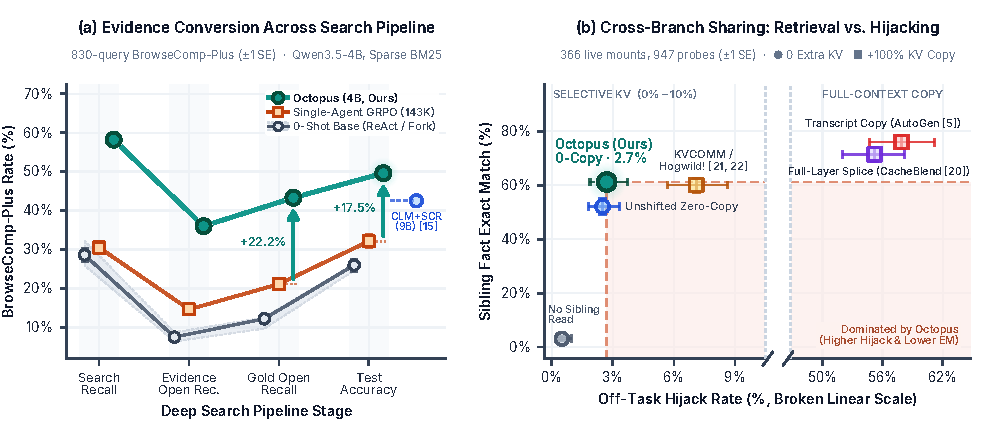
\includegraphics[width=0.95\textwidth]{figures/fig_exp2_efficiency.pdf}\vspace{-3pt}
\caption{Context conversion efficiency and cross-branch KV sharing on Qwen3.5-4B ($\pm 1\text{ SE}$). \textbf{(a)} Four-stage BrowseComp-Plus recall-to-accuracy pipeline ($830$ queries; per-query recall over $6.1$ evidence / $2.9$ gold docs, $58.9\%$ opening $\ge 1$ gold doc). \textbf{(b)} Sibling exact match vs.\ task hijacking across $366$ live \texttt{read\_thread} mounts ($947$ probes): \textbf{Octopus} retains $92.2\%$ answer information at $2.7\%$ hijacking with $0$ extra KV pages.}
\label{fig:efficiency-funnel}
\label{fig:mechanism-probe}
\end{figure}

\paragraph{Branch-Isolated Context Conversion, Evidence Grounding, and Radix Prefix Reuse.}
\Cref{fig:efficiency-funnel}(a) and \cref{tab:context-conversion} trace context conversion across the four BrowseComp-Plus stages (search, evidence-open, and gold-open recall, plus accuracy). Both $32\text{K}$ ReAct and 0-shot forking stall at $9.7\%$--$12.5\%$ gold-open recall ($20.7\%$ opening $\ge 1$ gold doc). Stretching a flat window to $143\text{K}$ under GRPO fails to unlock deeper search: with $0\%$ pruning of failed detours and noisy $8\text{K}$ pages, generated tokens bloat $3.9\times$ ($1{,}043 \to 4{,}075$) while usage stalls at $\mathbf{40.8\text{K}/143\text{K}}$ ($28.5\%$, $21.1\%$ gold-open recall).

By contrast, Octopus isolates sub-queries into clean $32\text{K}$ branches and prunes $38.8\%$ of post-initial steps via \texttt{rewind} ($61.4$ steps, $6.99$ rewinds/episode), keeping active prompts at $\mathbf{26.4\text{K}}$ tokens while exploring $\mathbf{329.2\text{K}}$ ($\mathbf{12.5\times}$ active; $541.3\text{K}$ on $\ge 250$-call queries) and retaining $\mathbf{199.0\text{K}}$ net tokens. Parallel execution compresses $19{,}251$ generated tokens into a $9{,}919$-token critical path ($\mathbf{1.94\times}$), lifting fractional gold-open recall from $21.1\%$ to $\mathbf{43.3\%}$ ($58.2\%$ search, $36.0\%$ evidence-open recall). Because BrowseComp-Plus annotates $2.89$ gold docs/query ($67.2\%$ multi-gold) and episodes stop once an opened gold page verifies the answer, Octopus opens $\ge 1$ gold doc on $\mathbf{58.9\%}$ of queries ($485/824$; $81.9\%$ conditional accuracy vs.\ $3.5\%$ otherwise): of $409$ correct answers ($49.6\%$), $\mathbf{97.1\%}$ ($397/409$) open $\ge 1$ gold doc and $2.4\%$ ($10/409$) open a non-gold evidence doc, while snippet-only answers drop from $25.3\%$ ($55/217$) at 0-shot to $\mathbf{0.5\%}$ ($2/409$) and zero-evidence parametric answers are $\mathbf{0.0\%}$ ($0/155$). At serving time, unlike in-place edits (CLM+SCR~\citep{shao2026clm}, $41.8\%$ edit re-prefill, breaking $\mathbf{h}_t$), Octopus reuses $\mathbf{89.59\%}$ of prompt tokens from GPU KV cache across $447{,}993$ H200 prefill batches ($14.56\text{B}$ vs.\ $1.69\text{B}$ prefilled), cuts wire traffic $\mathbf{98.3\%}$ ($662.3 \to 11.5\text{ MB}$), and speeds up $128\text{K}$ assembly $\mathbf{249\times}$ ($358.5 \to 1.44\text{ ms}$).

\begin{table}[!htb]
\centering
\caption{Per-episode context conversion efficiency on BrowseComp-Plus ($830$ queries) and server-resident radix prefix reuse across $447{,}993$ live H200 prefill batches.}
\label{tab:context-conversion}
\setlength{\tabcolsep}{5.6pt}
\setlength{\aboverulesep}{0pt}
\setlength{\belowrulesep}{0pt}
\renewcommand{\arraystretch}{1.13}
\resizebox{\textwidth}{!}{%
\begin{tabular}{lccccc}
\toprule
\rowcolor{hdrbg}
\hlcell{\textbf{Context Management}}{\textbf{\& Serving Architecture}} & \hcell{\textbf{Explored Context}}{\textbf{(Active / Win.\ Cap)}} & \hcell{\textbf{Critical-Path}}{\textbf{Token Load}} & \hcell{\textbf{Gold Open Rec.}}{\textbf{/ BCP Acc.\ $\uparrow$}} & \hcell{\textbf{GPU Prefix KV}}{\textbf{Cache Reuse $\uparrow$}} & \hcell{\textbf{128K Assembly}}{\textbf{\& Wire Cost $\downarrow$}} \\
\midrule
\rowstrut Single-Agent ReAct (Stateless $32\text{K}$) & $32.6\text{K}$ {\small($100\%$ of $32\text{K}$ cap)} & $1{,}043$ tok ($1.00\times$) & $12.2\%$ / $26.0\%$ & Append-only ($\mathcal{O}(L)$ resend) & $358.5\text{ ms}$ / $662.3\text{ MB}$ \\
\rowstrut Single-Agent GRPO (Flat $143\text{K}$ Window) & $40.8\text{K}$ {\small($28.5\%$ of $143\text{K}$ cap)} & $4{,}075$ tok ($3.9\times$ bloat) & $21.1\%$ / $32.1\%$ & Polluted window ($0\%$ pruned) & $358.5\text{ ms}$ / $662.3\text{ MB}$ \\
\rowstrut In-Place Context Edit (CLM+SCR, $9\text{B}$)~\citep{shao2026clm} & Multi-edit {\small($\le 32\text{K}$ active cap)} & $1.00\times$ serial edits & --- / $42.5\%$ {\scriptsize($1.34$ PF)} & $41.8\%$ edit re-prefill {\scriptsize(breaks $\mathbf{h}_t$)} & Suffix copy \& re-rotate \\
\rowcolor{oursrow}
\octotall{octo_radix}\slcell{\textbf{Octopus (Ours, $32\text{K}$ Branches)}}{{\small\color{ourstext}\textbf{Server-Resident Radix Cursor}}} & \scell{\textbf{$329.2\text{K}$ expl.\ / $199.0\text{K}$ net}}{{\small\color{ourstext}\textbf{($26.4\text{K}$ active; $541\text{K}$ hard)}}} & \scell{\textbf{$1.94\times$ compressed}}{{\small($9{,}919 / 19{,}251$ tok)}} & \scell{\textbf{$43.3\%$ / $49.6\%$}}{{\small\color{ourstext}\textbf{($58.9\%$ $\ge 1$ gold; $+22.2$)}}} & \scell{\textbf{$89.59\%$ GPU KV Hit}}{{\small($0\%$ prefix re-prefill)}} & \scell{\textbf{$1.44\text{ ms}$ ($249\times\uparrow$)}}{{\small($11.5\text{ MB}$, $-98.3\%$)}} \\
\bottomrule
\end{tabular}%
}
\end{table}

\paragraph{Hijack-Free Cross-Branch KV Mounting.}
\Cref{fig:efficiency-funnel}(b) and \cref{tab:kv-probe} benchmark cross-branch sharing across $366$ live \texttt{read\_thread} mounts on Qwen3.5-4B ($947$ exact-match identifier probes and $368$ fact-recall probes; in $52\%$ of mounts, sibling $A$ ran longer than reader $B$, $e_A > p_B$). Copying $A$'s transcript as text (\textbf{Transcript Copy}~\citep{wu2023autogen}) or splicing KV caches across all layers including recurrent states (\textbf{Full-Layer KV Splice}~\citep{yao2025cacheblend}) allocates $+100\%$ extra KV memory and steps $B$'s $24$ Gated DeltaNet states $\mathbf{h}_B$ through $A$'s tokens. As predicted in \cref{sec:method-cursor-mount}, overwriting $\mathbf{h}_B$ distorts $B$'s policy ($\Delta\text{NLL} = +0.195\text{--}0.196$) and hijacks $55.2\%$--$57.9\%$ of post-read turns into pursuing $A$'s sub-goal. Mounting attention KV without shifting positions (\textbf{Unshifted Zero-Copy KV}) avoids memory copies but drops from $0.612$ to $0.449$ exact match whenever $e_A > p_B$ due to inverted RoPE phases, whereas copying and re-rotating keys (\textbf{RoPE-Relocated KV Copy}~\citep{rodionov2025hogwild,ye2025kvcomm}) doubles KV memory and still incurs $7.1\%$ hijacking.

\textbf{Octopus Zero-Copy Mount} (\cref{eq:k2-pos}) splices sibling KV pages exclusively into the $8$ full-attention layers under monotonic position offsets while all $24$ recurrent layers skip the span: it allocates \textbf{$0$ extra KV pages}, retains $\mathbf{92.2\%}$ of full-text answer log-probability gain ($96.5\%$--$97.3\%$ fact recall) with no degradation on longer siblings ($0.613$ vs.\ $0.612$ exact match), cuts policy drift by $\mathbf{29\times}$ ($\Delta\text{NLL} = +0.007$), and reduces off-task hijacking by $\mathbf{21\times}$ ($57.9\% \to \mathbf{2.7\%}$). Across $115$ live rollouts, a blind judge finds no excess drift relative to a control that blocks the read ($\Delta\text{Hijack} = -1.1\%$), and the mechanism transfers cleanly to dense Transformers (Qwen3-4B, $\mathbf{96.9\%}$ argmax agreement) and Mamba-2 hybrids (Granite-4.0-H, $\mathbf{98.5\%}$; Appendix~\ref{app:arch-blueprints}).

\begin{table}[!htb]
\centering
\caption{Cross-branch context-sharing efficiency across $366$ live \texttt{read\_thread} mounts ($947$ probes on Qwen3.5-4B; $52\%$ with longer sibling $e_A > p_B$).}
\label{tab:kv-probe}
\setlength{\tabcolsep}{6.6pt}
\setlength{\aboverulesep}{0pt}
\setlength{\belowrulesep}{0pt}
\renewcommand{\arraystretch}{1.13}
\resizebox{\textwidth}{!}{%
\begin{tabular}{lccccc}
\toprule
\rowcolor{hdrbg}
\hlcell{\textbf{Cross-Branch Context-Sharing}}{\textbf{Mechanism}} & \hcell{\textbf{Extra KV}}{\textbf{Memory $\downarrow$}} & \hcell{\textbf{Full-Text Info}}{\textbf{Retained $\uparrow$}} & \hcell{\textbf{Exact Match $\uparrow$}}{{\scriptsize\textbf{All (Longer Sib.\ $e_A{>}p_B$)}}} & \hcell{\textbf{Policy Drift}}{\textbf{$\Delta$NLL $\downarrow$}} & \hcell{\textbf{Off-Task}}{\textbf{Hijack Rate $\downarrow$}} \\
\midrule
\rowstrut No Sibling Read (\texttt{none}) & $0$ Pages & $0.0\%$ {\small($62.5\%$ rec.)} & $0.031$ {\small($0.032$)} & $0.000$ & $0.5\%$ \\
\rowstrut Transcript Copy (AutoGen~\citep{wu2023autogen}) & $+100\%$ ($+L_{\text{mount}}$) & $\mathbf{100\%}$ {\small($\mathbf{99.5\%}$ rec.)} & $\mathbf{0.760}$ {\small($0.786$)} & $+0.196$ & $57.9\%$ \\
\rowstrut Full-Layer KV Splice (CacheBlend~\citep{yao2025cacheblend}) & $+100\%$ ($+L_{\text{mount}}$) & $98.1\%$ {\small($99.2\%$ rec.)} & $0.715$ {\small($0.731$)} & $+0.195$ & $55.2\%$ \\
\rowstrut Unshifted Zero-Copy KV & $0$ Pages ($0$-Copy) & $86.1\%$ {\small($94.3\%$ rec.)} & $0.521$ {\small($0.449$)} & $+0.003$ & $2.5\%$ \\
\rowstrut RoPE-Relocated KV Copy (KVCOMM~\citep{ye2025kvcomm,rodionov2025hogwild}) & $+100\%$ ($+L_{\text{mount}}$) & $91.7\%$ {\small($96.7\%$ rec.)} & $0.601$ {\small($0.611$)} & $+0.015$ & $7.1\%$ \\
\rowcolor{oursrow}
\octotall{octo_k2}\slcell{\textbf{Octopus Zero-Copy Mount (Ours)}}{{\small\color{ourstext}\textbf{Attn-Only Monotonic Offset (\cref{eq:k2-pos})}}} & \textbf{$0$ Pages ($0$-Copy)} & \scell{\textbf{$92.2\%$ Info}}{{\small($96.5\%$--$97.3\%$ rec.)}} & \scell{\textbf{$0.612$ {\small($0.613$)}}}{{\small\color{ourstext}\textbf{(0-shot: $0.627$)}}} & \scell{\textbf{$+0.007$}}{{\small($29\times\downarrow$ vs.\ Text)}} & \scell{\textbf{$2.7\%$ {\small($3.8\%$ 0-shot)}}}{{\small\color{ourstext}\textbf{($21\times\downarrow$ vs.\ Text)}}} \\
\bottomrule
\end{tabular}%
}\par\vspace{2.5pt}
\noindent\parbox{\textwidth}{\footnotesize
\textbf{Cross-Architecture Transfer:} Qwen3-4B (Dense, $9/36$L) $\mathbf{96.9\%}$ $\cdot$ Granite-4.0-H (Mamba-2 Hybrid) $\mathbf{98.5\%}$.\quad \textbf{Live Blind Audit ($115$ Reads):} $\Delta\text{Hijack} = \mathbf{-1.1\%}$ vs.\ Blocked-Read Control.}
\end{table}

\FloatBarrier
% ==============================================================================
% 4.3 MULTI-AGENT SCALABILITY (Figure 10 + Table 5)
% ==============================================================================
\subsection{Multi-Agent Scalability Across Agent Count and Tree Depth}
\label{sec:exp-scalability}
\label{sec:exp-topology}
\label{sec:exp-systems}

\begin{figure}[!htb]
\centering
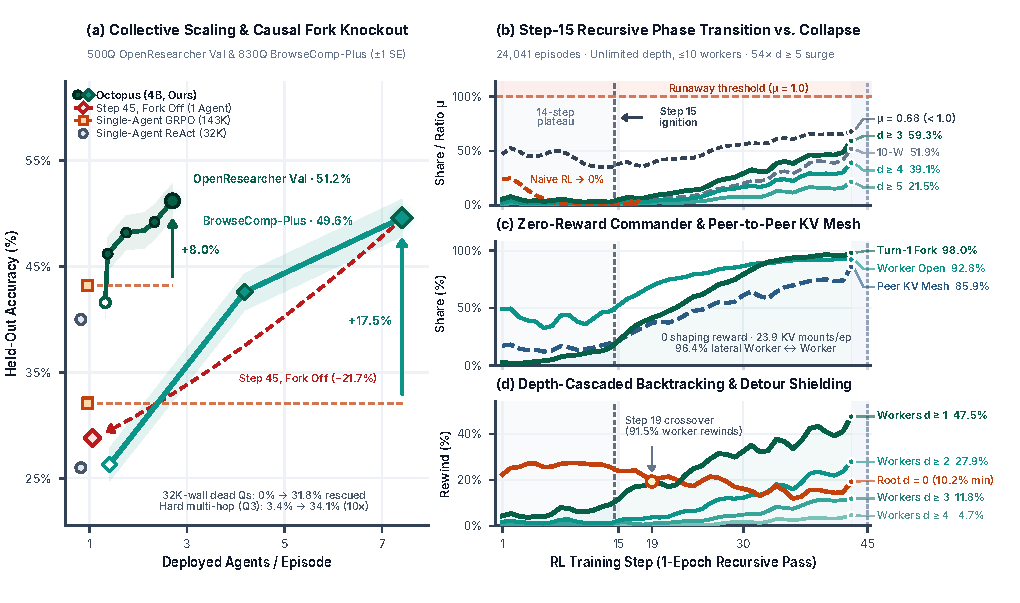
\includegraphics[width=0.97\textwidth]{figures/fig_exp3_agent_scaling.pdf}
\vspace{-5pt}
\caption{Multi-agent scaling and Step-$15$ recursive phase transition on Qwen3.5-4B. \textbf{(a)} Held-out accuracy vs.\ deployed agents per episode and same-weight \texttt{fork} knockout ($W_{\max}=0$, $\pm 1\text{ SE}$). \textbf{(b--d)} Unlimited-depth RL dynamics ($24{,}041$ episodes, $D_{\max}=\infty, W_{\max}=10$), showing sub-critical recursive scaling ($\mu < 1$), emergent peer-to-peer KV mounting, and depth-cascaded worker \texttt{rewind}s.}
\label{fig:topology-dynamics}
\vspace{-5pt}
\end{figure}

\paragraph{Scaling Accuracy with Deployed Agents and Causal Fork Knockout.}
\Cref{fig:topology-dynamics}(a) and \cref{tab:agent-scaling} track performance from a single linear thread ($W_{\max}=0$) to depth-$1$ parallel teams ($D_{\max}=1, W_{\max}=10$) and unlimited-depth hierarchies ($D_{\max}=\infty, W_{\max}=10$, up to $11$ threads/episode). Within $25{,}812$ depth-$1$ training rollouts, branched trajectories reach $61\%$--$66\%$ accuracy versus $52\%$ for unbranched rollouts on the same query, whereas rewinding an unbranched root yields no gain ($\Delta y = -0.014$); accordingly, DAG-GRPO drives root forking from $27\%$ to $98\%$ while cutting root rewinds $15\times$ ($0.413 \to 0.026$/episode). Held-out accuracy climbs monotonically with deployed agents per episode (\cref{fig:topology-dynamics}(a)): on OpenResearcher Validation, accuracy rises from $40.0\%$ ($32\text{K}$ ReAct) and $43.2\%$ ($143\text{K}$ GRPO) across $1.3$--$2.7$ agents/episode to $\mathbf{51.2\%}$ ($+8.0$ points); on BrowseComp-Plus, accuracy scales from $26.0\%$ ($32\text{K}$ ReAct) and $32.1\%$ ($143\text{K}$ GRPO) to $42.6\%$ at $4.18$ agents/episode ($D_{\max}=1$) and $\mathbf{49.6\%}$ at $\mathbf{7.41}$ agents/episode ($D_{\max}=\infty$, $6.41$ workers). Recursive branching rescues $\mathbf{31.8\%}$ ($116/365$) of queries that hit the $32\text{K}$ single-agent context wall ($0\%$ rescued at 0-shot) and boosts high-hop third-quartile (Q3) queries by $\mathbf{10\times}$ ($3.4\% \to 34.1\%$).

Crucially, we cap fanout at $W_{\max}=10$ only to match $9\text{B}$ single-agent RL compute ($2.00$ vs.\ $2.19\text{ PF/Q}$): episodes finishing naturally within $10$ workers ($69.2\%$, $570/824$) achieve $\mathbf{71.8\%}$ accuracy while $39.0\%$ hit the $10$-worker cap, indicating that scaling is budget-limited rather than saturated. Conversely, disabling \texttt{fork} at test time on the exact same Step~$45$ weights ($W_{\max}=0$) drops paired BrowseComp-Plus accuracy by $\mathbf{-21.7}$ points ($50.8\% \to 29.1\%$ across $571$ paired queries; $45.4\%$ on Validation), confirming that gains come from live multi-agent execution rather than single-thread weight distillation.

\paragraph{Step-15 Phase Transition, Emergent Peer KV Mesh, and 1D Training Scaling.}
Without our $1$-turn untrainable close reminder (Appendix~\ref{app:runtime-details}), naive $D_{\max}=\infty$ RL collapses from $28.2\%$ to $0\%$ forking within $15$ steps (\cref{fig:topology-dynamics}(b)). With the close contract ($24{,}041$ episodes over $45$ steps), Octopus plateaus for $14$ steps and then undergoes a sharp topological phase transition at Step~$15$: deep trees reaching $d \ge 3 / 4 / 5$ surge to $\mathbf{59.3\%} / \mathbf{39.1\%} / \mathbf{21.5\%}$ ($54\times$ increase at $d \ge 5$), yet the mean children spawned per worker remains sub-critical at $\mu \in [0.32, 0.69] < 1.0$, bounding expected tree size without depth caps ($6.41$ workers/episode on BrowseComp-Plus).

Driven solely by binary $0/1$ terminal rewards (\cref{fig:topology-dynamics}(c,d)), Step~$15$ simultaneously self-organizes three division-of-labor behaviors: \emph{(i)} Turn-$1$ root delegation jumps $38\times$ ($2.6\% \to \mathbf{98.0\%}$) while workers absorb $\mathbf{92.8\%}$ of $8\text{K}$ page \texttt{open} calls, keeping root contexts clean; \emph{(ii)} branches form a lateral \texttt{read\_thread} KV mesh ($17.3\% \to \mathbf{85.9\%}$ of episodes, averaging $\mathbf{23.9}$ zero-copy mounts/episode with $\mathbf{96.4\%}$ peer worker$\leftrightarrow$worker reads); and \emph{(iii)} past Step~$19$, root rewinds drop nearly $3\times$ ($29.3\% \to 10.2\%$ of episodes) as workers absorb $\mathbf{91.5\%}$ of all \texttt{rewind} calls ($47.5\%$ of episodes at $d \ge 1$ and $27.9\%$ at $d \ge 2$; Appendix~\ref{app:rollout-case}). Finally, 1D prefix-tree deduplication with live mounted KV edges (\cref{sec:method-kernels,sec:method-dag-grpo}) scales owned generated tokens trained per step by $\mathbf{8.1\times}$ on average ($\mathbf{11.1\times}$ peak, $101.6\text{K} \to 1.12\text{M}$ tokens/step, $0$ OOM) while holding rollout--training divergence at $\mathrm{KL}(\pi_{\text{rollout}} \parallel \pi_\theta) = 4.45 \times 10^{-4}$---$\mathbf{32\times}$ lower than dropping mounted KV edges ($0.0142$).

\begin{table}[!htb]
\centering
\caption{Multi-agent scalability across worker budget ($W_{\max}$), recursive tree depth ($D_{\max}$), and emergent division of labor on Qwen3.5-4B.}
\label{tab:agent-scaling}
\label{tab:topology-ablation}
\label{tab:h200-systems}
\setlength{\tabcolsep}{4.2pt}
\setlength{\aboverulesep}{0pt}
\setlength{\belowrulesep}{0pt}
\renewcommand{\arraystretch}{1.15}
\resizebox{\textwidth}{!}{%
\begin{tabular}{llcccccc}
\toprule
\rowcolor{hdrbg}
\hlcell{\textbf{Multi-Agent Topology}}{\textbf{\& Training Regime}} & \hlcell{\textbf{Max Threads}}{\textbf{(Depth, Fanout)}} & \hcell{\textbf{Root}}{\textbf{Fork Rate}} & \hcell{\textbf{Workers / Ep}}{\textbf{(Child Ratio $\mu$)}} & \hcell{\textbf{Deep ($d{\ge}3$)}}{\textbf{/ Full 10-Br.}} & \hcell{\textbf{Rewind Activity}}{\textbf{(Root / Worker)}} & \hcell{\textbf{OpenResearcher}}{\textbf{Acc.\ $\uparrow$}} & \hcell{\textbf{BCP Test}}{\textbf{Acc.\ $\uparrow$}} \\
\midrule
\rowstrut Single-Agent ReAct ($32\text{K}$ Window) & $1$ ($0, 0$) & $0\%$ & $0.00$ ($0.00$) & $0\%$ / $0\%$ & --- / --- & $40.0\%$ {\small(Val)} & $26.0\%$ \\
\rowstrut Single-Agent GRPO ($143\text{K}$ Flat) & $1$ ($0, 0$) & $0\%$ & $0.00$ ($0.00$) & $0\%$ / $0\%$ & --- / --- & $43.2\%$ {\small(Val)} & $32.1\%$ \\
\rowstrut Multi-Agent Fork (0-Shot Base) & $\le 11$ ($\infty, 10$) & $11\%$ {\scriptsize($16\%$ Val)} & $0.41$ {\scriptsize($0.32$ Val)} & $0\%$ / $0\%$ & $1.51$ rw/ep {\scriptsize($9.7$ st)} & $41.6\%$ {\small(Val)} & $26.3\%$ {\scriptsize($24.8\%$)} \\
\rowcolor{oursrow}
\octodense{octo_17_rewind_cut}\textbf{Octopus RL (Parallel Team, $D_{\max}{=}1$, Step 35)} & $\le 11$ ($1, 10$) & \good{$92\%$} & \good{$3.18$ ($0.00$)} & $0\%$ / $0.2\%$ & $0.29$/ep / $0.52$/br & \good{$46.5\%$ {\small(Val)}} & \good{$42.6\%$ \gain{+10.5}} \\
\rowcolor{oursrowdeep}
\octodense{octo_fork}\textbf{Octopus RL (Parallel Team, $D_{\max}{=}1$, Step 55)} & $\le 11$ ($1, 10$) & \best{$98\%$} & \best{$1.70$ ($0.00$)} & $0\%$ / $0.6\%$ & \best{$0.026$/ep / $0.24$/br} & \best{51.2\% {\small(Val)}} & --- \\
\rowstrut Recursive 0-Shot ($D_{\max}{=}\infty$ on $D_{\max}{=}1$ Policy) & $\le 11$ ($\infty, 10$) & $97\%$ & $2.34$ ($0.27$) & $8.6\%$ / --- & --- / --- & $44.4\%$ {\small($57.2\%^\ddagger$)} & --- \\
\rowcolor{oursrow}
\octodense{octo_20_commit_gate}\textbf{Octopus RL (Recursive, $D_{\max}{=}\infty$, Step 20)} & $\le 11$ ($\infty, 10$) & \good{$55\%$} & \good{$1.15$ ($0.46$)} & $11.4\%$ / $8.9\%$ & $23.7\%$ / $18.6\%$ {\scriptsize ep} & \good{$46.6\%$ {\small(Val)}} & --- \\
\rowcolor{oursrow}
\octodense{octo_17_rewind_cut}\textbf{Octopus RL (Recursive, $D_{\max}{=}\infty$, Step 43 Rollout$^\ddagger$)} & $\le 11$ ($\infty, 10$) & \good{$99.2\%$} & \good{$6.85$ ($0.68$)} & \best{$59.3\%$ / $51.9\%$} & \best{$10.2\%$ / $47.5\%$ {\scriptsize ep}} & \good{$57.9\%$ {\small(Train$^\ddagger$)}} & --- \\
\rowcolor{oursrowdeep}
\octodense{octo_15_search_king}\textbf{Octopus RL (Recursive, $D_{\max}{=}\infty$, Step 45, $1$-Ep.)} & $\le 11$ ($\infty, 10$) & \best{$99.5\%$} & \best{$6.41$ {\small($7.41$ ag.)}} & --- / \best{$39.0\%$} & \best{$6.99$ rw/ep {\scriptsize($61.4$ st)}} & \good{$45.4{\to}46.5\%$ {\scriptsize($W{\le}1^\ddagger$)}} & \best{49.6\% \gain{+17.5}} \\
\midrule
\rowcolor{hdrbg}
\multicolumn{8}{l}{\rowstrut{\footnotesize\textbf{1D Prefix-Tree Deduplication (\cref{sec:method-kernels}):} $\mathbf{8.1\times}$ avg ($\mathbf{11.1\times}$ peak, $101.6\text{K}{\to}1.12\text{M}$ tok/step, $0$ OOM).\quad \textbf{On-Policy Mount KL:} $\mathbf{4.45{\times}10^{-4}}$ (vs.\ $0.0142$ w/o mounts, $\mathbf{32\times\downarrow}$).}} \\
\bottomrule
\end{tabular}%
}\par\vspace{3.0pt}
\noindent\parbox{\textwidth}{\footnotesize
$^\ddagger$Zero-shot $D_{\max}=\infty$ transfer of the $D_{\max}=1$ policy scores $44.4\%$ across all $500$ Val queries ($222/500$) and $57.2\%$ on completed trees ($222/388$). Step~$43$ reports late-training rollout statistics ($57.9\%$ training rollout accuracy); at Step~$45$ ($1$ epoch = $3{,}040$ queries), restricting test-time fanout on Val to $W_{\max}=0 / 1$ yields $45.4\% / 46.5\%$, while full recursive evaluation ($W_{\max}=10$) reaches $\mathbf{49.6\%}$ on BrowseComp-Plus.}
\vspace{-4pt}
\end{table}
\FloatBarrier

% ==============================================================================
\section{Conclusion and Limitations}
\label{sec:discussion}

Long-horizon reasoning agents need not be confined to a single append-only text window. \textbf{Octopus} recasts agentic execution as a stateful, GPU-resident DAG in which branches fork and backtrack over reference-counted radix KV prefixes and recurrent checkpoints in $\mathcal{O}(1)$ zero copy, while exchanging findings directly through attention-only KV mounting without overwriting private recurrent working memory ($92.2\%$ information retention, $21\times$ lower task hijacking, $89.6\%$ live GPU KV hit rate). Trained end-to-end with 1D packed DAG-GRPO under pure binary outcome rewards and zero process shaping, a $4\text{B}$ sparse-BM25 model self-organizes a sub-critical commander--mesh hierarchy---reaching $49.6\%$ on BrowseComp-Plus ($+17.5$ points over $143\text{K}$ single-agent RL; $-21.7$ points when test-time \texttt{fork} is disabled on the same weights) and $51.2\%$ on OpenResearcher, outperforming dense-retriever systems up to $250\times$ larger. These results establish latent-space multi-agent branching as an effective scaling axis orthogonal to model parameters and single-window length.

\paragraph{Limitations and Future Directions.}
Our current study trains a single homogeneous backbone over episode-scoped KV cursors within single-node GPU pools (up to $524$ resident cursors/GPU at $W_{\max}=10$, with tree-size loss normalization $1/Z_i$), opening three broader directions. First, \textbf{heterogeneous multi-model branching}: while our runtime already supports seven dense, MoE, and hybrid families (Appendix~\ref{app:arch-blueprints}), each episode currently executes one shared model; routing sub-branches across role-specialized LoRA adapters or heterogeneous model scales---such as lightweight scout branches paired with heavyweight verifiers via learned KV projections---could markedly improve compute--accuracy trade-offs. Second, \textbf{persistent LoRA and latent long-term memory}: mounted KV pages are currently reclaimed at episode end; consolidating verified branch KV states into persistent cross-episode memory banks or continual LoRA weights would extend Octopus from episodic reasoning to lifelong agentic memory. Third, \textbf{million-agent collective scaling}: tiering reference-counted radix cursors and recurrent checkpoints across GPU HBM, host DRAM/NVMe, and multi-node RDMA fabrics would scale latent-space coordination from ten-branch trees to asynchronous million-agent swarms.

{\setlength{\parskip}{0pt}
\renewcommand{\bibfont}{\fontsize{7.8pt}{8.9pt}\selectfont}
\setlength{\bibsep}{0pt}
\bibliographystyle{unsrtnat}
\bibliography{references}
}

\clearpage
\appendix
\setlength{\parskip}{3.5pt plus 0.6pt minus 0.3pt}
\section{Cross-Family Chat-Template Probing and Runtime Guardrails}
\label{app:runtime-details}

\paragraph{Automatic Startup Chat-Template Probing and Tagged Injections.}
Open-weight chat templates $\mathcal{T}$ frequently violate strict append-only rendering: Qwen2.5/3/3.5 strip earlier assistant reasoning blocks upon a new user turn, DeepSeek-V3/R1 format initial and subsequent tool calls asymmetrically, Mistral-v0.3 embeds the system prompt inside the final user turn, and gpt-oss drops analysis channels on re-render. At server startup ($\sim 0.1\,\text{s}$), Octopus probes synthetic $(\text{parent-reply}, \text{delta-turn})$ pairs to locate the assistant-turn terminator $\tau_{\text{term}}$ and classify $\mathcal{T}$ into one of two incremental delta modes (\cref{sec:method-cursor-mount}). Templates with history-invariant suffixes use a \emph{constant stub} that slices $\mathrm{Render}_\Delta$ directly after $\tau_{\text{term}}$ (covering Qwen, Llama-3, DeepSeek-V3.1, and GLM-4.5/4.7), whereas context-sensitive templates render against a \emph{minimal context stub} $\mathrm{ctx}(c)$ before slicing (covering DeepSeek-V3/R1, Mistral-v0.3, and gpt-oss), yielding $0 / 18{,}344$ tokenization mismatches. Mid-episode runtime notifications (\texttt{fork}, join, and \texttt{rewind} notes) are injected as tagged tool responses rather than user turns so prior reasoning blocks remain intact.

\paragraph{Append-Only \texttt{read\_thread} Injection, Answer Reserve, and Eviction Rebuild.}
To preserve $100\%$ shared prefix KV caching while preventing pre-fork self-reads, Octopus omits \texttt{read\_thread} from the static system prompt and appends its tool specification and sibling roster only after a readable peer step exists, clamping requested step ranges $[s, e]$ to the source's valid steps $[A, B]$ via $[\max(s, A), \min(e, B)]$. Within each thread's $B_{\text{thread}} = 32{,}768$-token growth budget, $R_{\text{ans}} = 2{,}048$ tokens are reserved for final synthesis, and tool-less plain-text replies trigger a single untrainable close reminder ($m_{\ell,t}=0$). Completed cursors store compact mount-breakpoint tables in a server-side LRU registry, while mounted KV spans link into the GPU radix tree through negative placeholder token IDs and per-page reference counts. If GPU memory pressure or an online LoRA weight update evicts a mounted segment, the server aborts before token emission and executes a batched zero-decode prefill rebuild from the cursor's breakpoint table.

\paragraph{KV-Aware Episode Admission and Branch Turn Budget.}
Gating new episode admission on live server KV pool utilization ($\tau_{\text{KV}} = 0.75$ with zero waiting queue) prevents mid-episode fork bursts from saturating GPU memory (\cref{sec:exp-scalability}). Whereas unbounded dispatch drives P90 KV utilization to $98\%$--$99\%$ ($72$--$88$ queued requests) and causes $14.7\%$--$46.1\%$ episode timeouts, the $75\%$ gate caps P90 KV load at $74.5\%$ ($0$ queued, $0 / 1{,}304$ timeouts). This allows each $141\text{GB}$ GPU ($1.94\text{M}$-token KV pool) to host up to $524$ resident GDN recurrent checkpoints and $154$ concurrently decoding threads at $1{,}044.5\text{ tok/s}$ (P90). In addition, raising the per-branch turn cap from $T_{\text{br}}=20$ to $T_{\text{br}}=50$ prevents rewound branches from exhausting their turn budget before calling \texttt{done}, narrowing the completion-rate gap between rewound and unrewound branches ($\Delta\text{Done}$) from $-36.0\%$ ($95\%$ CI: $[-42.2\%, -29.4\%]$) to $-4.1\%$.

\paragraph{Closing-Contract Guardrail Against Policy Collapse.}
We further compare three episode-closing contracts across $33{,}075$ pooled unlimited-depth rollouts ($D_{\max}=\infty, W_{\max}=10$, combining our $24{,}041$-episode main run with two baseline-contract runs). Under \emph{fallback plain-text grading}, scoring tool-less root replies via answer extraction causes unverified tool-less endings to surge from $6\%$ to $75\%$ by Step~$12$ ($41\%$ at $d \ge 3$). Conversely, under \emph{strict \texttt{done}-only grading without a reminder}, the $7.5\%$ of forked roots that emit plain text after a join note receive zero reward ($y=0$), assigning negative advantage to forking ($\hat{A}_{\text{fork}} = -0.044$) and collapsing root fork rates from $23.9\%$--$28.2\%$ to $0\%$ at Step~$15$ ($1.2\%$ at Step~$17$; \cref{fig:topology-dynamics}(b)). Injecting our single-turn untrainable close reminder ($m_{\ell,t}=0$) converts $97.4\%$ of reminded roots and $93.1\%$ of reminded sub-branches into valid \texttt{done} calls ($0.2\%$ tool-less), sustaining $98.8\%$--$99.2\%$ root forking across the full $45$-step training pass.

\section{Concrete Unlimited-Depth Search Rollout Walkthrough (\texttt{search-3190-99})}
\label{app:rollout-case}

To illustrate how Octopus's five execution primitives, layer-selective KV mounting, and sub-critical unlimited-depth tree execution work together on a long-horizon episode, \cref{fig:search-rollout-case} and \cref{tab:rollout-walkthrough} trace a real evaluation episode (\texttt{search-3190-99}) on the multi-hop query: \emph{``During a late twentieth-century volcanic event in the Luzon Volcanic Arc that was notable for lowering global temperatures for several years and having an ash cloud significantly larger than the 1980 eruption of a U.S.\ mountain, how many commercial airplanes experienced in-flight damage as a result of inadvertently entering the airborne particulate cloud generated by this eruption? Answer with a whole number only.''}

\begin{figure}[!t]
\centering
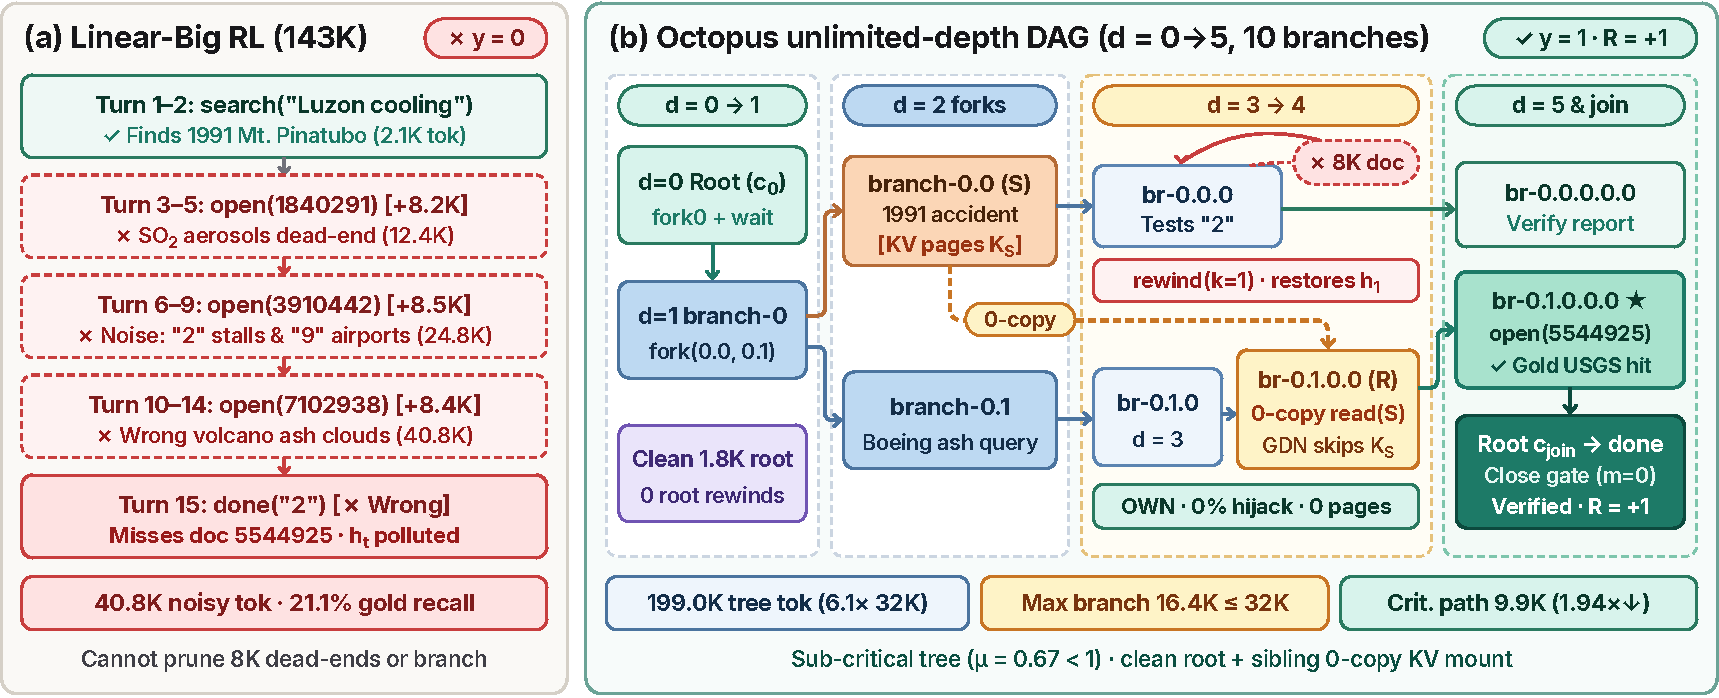
\includegraphics[width=1.0\textwidth]{figures/fig_search_rollout_case.pdf}
\caption{Multi-hop search rollout case study (\texttt{search-3190-99}: 1991 Mt.\ Pinatubo ash-cloud aircraft damage). \textbf{(a)} Flat $143\text{K}$ single-thread RL ($32.1\%$ BCP) accumulates noisy retrieval detours inside one append-only context, polluting its recurrent state $\mathbf{h}_t$. \textbf{(b)} Under $D_{\max}=\infty, W_{\max}=10$, Octopus ($49.6\%$ BCP, $57.9\%$ Rollout) keeps the root clean ($1.8\text{K}$ tok) while spawning a depth-$5$, $10$-branch DAG ($\mu = 0.67 < 1$): dead-end queries are pruned via branch \texttt{rewind}, and \texttt{branch-0.1.0.0} ($d=4$) zero-copy mounts sibling \texttt{branch-0.0}'s attention KV pages ($0\%$ hijack) before opening \texttt{docid=5544925} at $d=5$.}
\label{fig:search-rollout-case}
\par\vspace{9pt}
\captionsetup{type=table, skip=5.5pt}
\captionof{table}{Step-by-step trace and hybrid recurrent/attention state transitions for unlimited-depth rollout \texttt{search-3190-99} ($D_{\max}=\infty, W_{\max}=10$, $10$ branches across $d=0 \to 5$).}
\label{tab:rollout-walkthrough}
\footnotesize
\setlength{\tabcolsep}{4.5pt}
\setlength{\aboverulesep}{0pt}
\setlength{\belowrulesep}{0pt}
\renewcommand{\arraystretch}{1.05}
\resizebox{\textwidth}{!}{%
\begin{tabular}{L{2.45cm} L{8.15cm} L{7.90cm}}
\toprule
\rowcolor{hdrbg}
\tstrut\textbf{Depth \& Cursor}\bstrut & \tstrut\textbf{Agent Trajectory (Prompt / Thought / Tool Call \& Return)}\bstrut & \tstrut\textbf{GPU Radix Cursor, Hybrid State \& DAG-GRPO Semantics}\bstrut \\
\midrule
\rowcolor{oursrow}
\tstrut\textbf{$d=0$ Root}\newline$c_0 \to \texttt{fork0}$\newline{\scriptsize(Orchestrator)}\bstrut &
\tstrut\textbf{Thought:} Identify 1991 Mt.\ Pinatubo (Luzon Arc) and delegate commercial aircraft damage lookup.\newline
\textbf{Call:} \texttt{fork(\{"branch-0": "find number of commercial airplanes that experienced in-flight damage from Mount Pinatubo 1991 ash cloud"\})} $+$ \texttt{wait(["branch-0"])}\bstrut &
\tstrut\cmarkyes~\textbf{$\mathcal{O}(1)$ Zero-Copy Spawn:} Increments Radix KV ref-count at $c_{\text{fork}}$ by $+1$; clones GDN recurrent state $\mathbf{h}_{\text{end}}(c_0)$.\newline
\cmarkyes~\textbf{Clean Orchestrator:} Root suspends at $1.8\text{K}$ tok; \texttt{branch-0} gets fresh $B_{\text{thread}} = 32\text{K}$ cap.\bstrut \\
\midrule
\tstrut\textbf{$d=1 \to 2$ Fork}\newline\texttt{branch-0}\newline$\to$ \texttt{0.0} ($S$), \texttt{0.1}\bstrut &
\tstrut\textbf{Call ($d=1$):} \texttt{search("Mount Pinatubo 1991 ash cloud commercial airplanes damage")} $\to$ surfaces ``more than 20 airplanes'' and ``24 windshields'', then sub-forks ($d=2$):\newline
$\bullet$ \texttt{branch-0.0} ($S$): \texttt{"search for Pinatubo 1991 aircraft accident airplanes"}\newline
$\bullet$ \texttt{branch-0.1}: \texttt{"search for \textbackslash"Pinatubo\textbackslash" Boeing airplanes ash"}\bstrut &
\tstrut\cmarkyes~\textbf{Recursive Expansion ($D_{\max}=\infty$):} Each $d=2$ child shares parent KV prefix in $\mathcal{O}(1)$ and inherits $\mathbf{h}_{\text{end}}(\texttt{branch-0})$.\newline
\cmarkyes~\textbf{Hypothesis Isolation:} Sibling $S$ (\texttt{branch-0.0}) extracts candidate docID \texttt{5544925} and encounter tables into its KV pages.\bstrut \\
\midrule
\rowcolor{badcell}
\tstrut\textbf{$d=3 \to 5$ Left}\newline\texttt{branch-0.0.0*}\newline{\scriptsize\color{badtext}(Dead-End Path)}\bstrut &
\tstrut\textbf{Sub-Forks:} \texttt{0.0.0} ($d=3$: \texttt{"...damage 2"}) $\to$ \texttt{0.0.0.0} ($d=4$) $\to$ \texttt{0.0.0.0.0} ($d=5$).\newline
\textbf{Dead End \& Rewind:} Queries on ``2 crashes'' open noisy incident pages ($+8.4\text{K}$ tok); branch calls \texttt{rewind(step=1, note="2 is engine replacements; pivot to USGS report")}.\bstrut &
\tstrut\cmarkyes~\textbf{Branch Rewind:} Cursor resets to $c_1$ (reclaiming $+8.4\text{K}$ of $B_{\text{thread}}$); GDN layers restore exact $\mathbf{h}_1$ (erasing dead-end noise).\newline
\cmarkyes~\textbf{Single-Ownership (\cref{sec:method-dag-grpo}):} Dead-end leaf kept in DAG so \texttt{rewind} gets RL credit; post-rewind masks $m_{\ell,t}=0$ ($t \le 1$).\bstrut \\
\midrule
\rowcolor{oursrowdeep}
\tstrut\textbf{$d=3 \to 4$ Right}\newline\texttt{branch-0.1.0.0}\newline{\scriptsize(Reader $R$)}\bstrut &
\tstrut\textbf{Sub-Forks:} \texttt{branch-0.1.0} ($d=3$: \texttt{"...\textbackslash"airplanes\textbackslash" 24 windshields"}) spawns $d=4$ siblings \texttt{0.1.0.0} ($R$) and \texttt{0.1.0.1}.\newline
\textbf{Cross-Branch Mount:} Reader $R$ (\texttt{branch-0.1.0.0}) invokes \texttt{read\_thread(branch="branch-0.0", steps=[1, 3])} to inspect sibling $S$'s retrieval table without re-searching.\bstrut &
\tstrut\good{\cmarkyes~Hijack-Free Zero-Copy KV Mount (\cref{eq:k2-pos}):}\newline
$\bullet$ \textbf{Full-Attention Layers:} Borrow $S$'s physical KV pages ($0$ new pages); $R$'s next token jumps to $s(c_R') = \max(p_R, e_S+1)$.\newline
$\bullet$ \textbf{GDN Recurrent Layers:} Skip stepping over mounted span; $\mathbf{h}_R$ advances only along $R$'s post-mount tokens (\textbf{retains own sub-task, $0\%$ hijack}).\bstrut \\
\midrule
\rowcolor{oursrow}
\tstrut\textbf{$d=5$ Leaf \& Join}\newline\texttt{0.1.0.0.0} $\to c_{\text{join}}$\newline{\scriptsize(Verify \& Close)}\bstrut &
\tstrut\textbf{Leaf Verification ($d=5$):} $R$ spawns \texttt{branch-0.1.0.0.0} (\texttt{"open 5544925 offset 0"}), verifying the primary USGS/ICAO ash report, and closes via \texttt{done}.\newline
\textbf{Root Synthesis ($d=0$):} \texttt{wait} returns at $c_{\text{join}}$; runtime injects $1$-turn Close Reminder ($m_{\ell,t}=0$), and root calls \texttt{done} with exact whole-number answer.\bstrut &
\tstrut\cmarkyes~\textbf{Sub-Critical Tree Growth (\cref{sec:exp-topology}):} Terminates at $W=10$ branches ($1,2,2,3,2$ at $d=1..5$; empirical $\mu = 0.67 < 1$).\newline
\cmarkyes~\textbf{On-Policy Mount Retention (\cref{eq:dag-attn,eq:lora-kv}):} Keeps mounted $\mathbf{K}_S, \mathbf{V}_S$ in the 1D packed forward--backward graph.\bstrut \\
\bottomrule
\end{tabular}%
}
\end{figure}
\FloatBarrier

\section{Per-Architecture Framework Integration Blueprints}
\label{app:arch-blueprints}

Octopus supports dense, sparse-MoE, and hybrid recurrent-attention model families across both serving and 1D prefix-tree RL through a declarative architecture registry paired with automatic serving-engine LoRA target resolution (\cref{tab:arch-hooks}).

\paragraph{Pure Full-Attention Dense and Sparse-MoE Transformers (\texttt{Qwen3 Dense}, \texttt{Llama-3}, \texttt{Qwen3 MoE}).}
In models composed solely of full, sliding, or chunked attention with no recurrent state ($\mathbf{h}_t = \emptyset$), \texttt{fork} and \texttt{rewind} reduce to $\mathcal{O}(1)$ PagedAttention radix pointer updates. Because pure-attention models lack private recurrent layers to anchor branch identity, mounting sibling KV pages across all $L$ layers can induce cross-branch persona drift; Octopus therefore mounts $c_A[s:e)$ under monotonic position offsets (\cref{eq:k2-pos}) into only a sparse subset of middle retrieval layers ($\mathcal{L}_{\text{mount}} \subset \{1,\dots,L\}$, e.g., $9/36$ layers in Qwen3-4B-Base) while presenting a mount-free KV view to the remaining $27$ layers. This middle-layer mounting retains $96.9\%$ argmax agreement with full-context replay during serving, while the 1D packed trainer dispatches separate variable-length FlashAttention passes for mounted and unmounted layer groups (\cref{tab:arch-hooks}). For sparse Mixture-of-Experts models (\texttt{Qwen3 MoE}), token-wise Top-$K$ routing ($K=8$) carries no cross-position state, so branching incurs zero expert-state copies and 1D prefix-tree deduplication batches active branches into a single grouped GEMM pass.

\paragraph{Hybrid Recurrent-Attention Architectures (\texttt{Qwen3.5 GDN} and \texttt{Granite-4.0-H Mamba-2}; \cref{fig:arch-hybrid}).}
In Qwen3.5 ($8$ blocks of three Gated DeltaNet layers and one Gated Full-Attention layer; \cref{fig:arch-hybrid}(a)), all $8$ full-attention layers zero-copy mount sibling KV pages under \cref{eq:k2-pos} (denoted Rule~K2 in \cref{fig:arch-hybrid}) prior to the output sigmoid gate, whereas all $24$ GDN layers clone or restore $\mathbf{h}_k$ on \texttt{fork}/\texttt{rewind} and skip mounted spans. During 1D packed DAG-GRPO training, tree-boundary hooks gather $d_{\text{conv}} - 1 = 3$ ancestor tokens for short causal convolutions and run level-by-level variable-length GDN recurrence via FlashLinearAttention (\texttt{fla}) initialized from each node's parent checkpoint $\mathbf{h}_{\text{end}}(p(u))$. Activation tiling in $16\text{K}$-token chunks prevents backward memory spikes on trees spanning up to $262\text{K}$ tokens, while fused projection LoRA adapters (\cref{tab:arch-hooks}) align PEFT gradients directly with SGLang serving weights. Analogously, for Mamba-2 + GQA hybrids (\texttt{Granite-4.0-H}; \cref{fig:arch-hybrid}(b)), Octopus maps Mamba-2 Structured State Space Duality (SSD) onto \texttt{fla}'s chunked linear-attention kernels with ancestor convolution gathering and supports recursive transitive KV mounting ($X \leadsto A \leadsto C$, $98.5\%$ token agreement).

\begin{table}[!t]
\centering
\caption{Per-architecture integration hooks across model families in \texttt{octopus/rl/model\_hooks.py}, \texttt{lora\_targets.py}, \texttt{seq\_tiles.py}, and \texttt{patches/apply\_sglang\_*.py}. Unregistered stateful architectures raise an explicit startup guard.}
\label{tab:arch-hooks}
\footnotesize
\setlength{\tabcolsep}{4.0pt}
\setlength{\aboverulesep}{0pt}
\setlength{\belowrulesep}{0pt}
\renewcommand{\arraystretch}{1.10}
\resizebox{\textwidth}{!}{%
\begin{tabular}{L{3.10cm} L{3.55cm} L{4.10cm} L{4.45cm} L{4.45cm}}
\toprule
\rowcolor{hdrbg}
\tstrut\textbf{Architecture Family}\bstrut & \tstrut\textbf{Decoder Layer Topology}\bstrut & \tstrut\textbf{Serving KV Mount \& State Hook}\bstrut & \tstrut\textbf{Prefix-Tree Recurrence, Conv \& Tiling Hook}\bstrut & \tstrut\textbf{SGLang-Resolved LoRA Targets (\texttt{lora\_targets.py})}\bstrut \\
\midrule
\rowcolor{oursrow}
\tstrut\textbf{\texttt{Qwen3 (Dense)}}\newline{\scriptsize(\texttt{qwen3}, \texttt{llama3})}\bstrut &
\tstrut$L$ Full-Attn + SwiGLU MLP ($\mathcal{L}_{\text{rec}} = \emptyset$)\bstrut &
\tstrut\texttt{OCTOPUS\_MOUNT\_LAYERS} ($9/36$ layers mount $c_A[s:e)$; $27$ call \texttt{hide\_mounts})\bstrut &
\tstrut$\texttt{CONV\_CONTEXT} = 0$; varlen FlashAttn \texttt{attn\_calls} vs.\ \texttt{own\_calls} ($32\text{K}$ chunks)\bstrut &
\tstrut$7$ modules: \texttt{q\_proj, k\_proj, v\_proj, o\_proj, gate\_proj, up\_proj, down\_proj}\bstrut \\
\midrule
\tstrut\textbf{\texttt{Qwen3 (MoE)}}\newline{\scriptsize(\texttt{qwen3\_moe})}\bstrut &
\tstrut$L$ Full-Attn + Top-$K$ Sparse MoE ($K=8$)\bstrut &
\tstrut Attention-only Radix KV mount + \cref{eq:k2-pos} jump; $0$ MoE state on \texttt{fork}/\texttt{rewind}\bstrut &
\tstrut$\texttt{CONV\_CONTEXT} = 0$; 1D deduplicated tree tokens $T_{\text{tree}}$ batched into MoE grouped GEMM\bstrut &
\tstrut Attention LoRA (\texttt{q/k/v/o\_proj}); preserves Top-$K$ router gate stability\bstrut \\
\midrule
\rowcolor{oursrowdeep}
\tstrut\textbf{\texttt{Qwen3.5 (Dense)}}\newline{\scriptsize(\texttt{qwen3\_5}, Primary)}\bstrut &
\tstrut$8 \times [3\text{ GDN} + 1\text{ Gated Attn}]$ ($24$ GDN, $8$ Attn) + SwiGLU MLP\bstrut &
\tstrut All $8$ Full-Attn layers 0-copy mount $c_A[s:e)$; $24$ GDN layers clone/restore $\mathbf{h}_k$ \& skip mounts\bstrut &
\tstrut$\texttt{CONV\_CONTEXT} = d_{\text{conv}}-1 = 3$ (\texttt{tree\_conv}); \texttt{fla} \texttt{chunk\_gated\_delta\_rule}; \texttt{TILE=16K} (\texttt{seq\_tiles.py})\bstrut &
\tstrut$10$ modules: \texttt{q/k/v/o\_proj, gate/up/down\_proj, out\_proj} + fused \texttt{in\_proj\_qkvz}\bstrut \\
\midrule
\rowcolor{oursrow}
\tstrut\textbf{\texttt{Qwen3.5-MoE / Next}}\newline{\scriptsize(\texttt{qwen3\_5\_moe}, \texttt{qwen3\_next})}\bstrut &
\tstrut$24$ GDN + $8$ Gated Attn + Sparse Top-$K$ MoE (+ Shared Expert)\bstrut &
\tstrut$8$ Full-Attn layers mount $c_A[s:e)$; $24$ GDN layers skip mounted spans; $0$ MoE state overhead\bstrut &
\tstrut$\texttt{CONV\_CONTEXT} = 3$ (\texttt{tree\_conv}) + level-by-level \texttt{tree\_recurrence} ($32\text{K}$ segs); HF MoE forward\bstrut &
\tstrut Attention + GDN projections (\texttt{q/k/v/o\_proj, in\_proj\_qkvz, out\_proj})\bstrut \\
\midrule
\tstrut\textbf{\texttt{Granite-4.0-H}}\newline{\scriptsize(\texttt{granitemoehybrid})}\bstrut &
\tstrut Mamba-2 SSD Mixer + GQA Full-Attn + Sparse MoE \& Shared MLP\bstrut &
\tstrut Transitive $X \leadsto A \leadsto C$ Attn KV mount ($98.5\%$ agree); Mamba-2 state $\mathbf{h}_k$ skips mounts; 1$\times$ final norm patch\bstrut &
\tstrut$\texttt{CONV\_CONTEXT} = \texttt{mamba\_d\_conv}-1$ (\texttt{tree\_conv}); SSD mapped to \texttt{fla} \texttt{chunk\_simple\_gla}\bstrut &
\tstrut$5$ modules: \texttt{q\_proj, k\_proj, v\_proj, o\_proj} + patched Mamba \texttt{out\_proj} ($H\cdot P \to D$)\bstrut \\
\bottomrule
\end{tabular}%
}
\par\vspace{11pt}
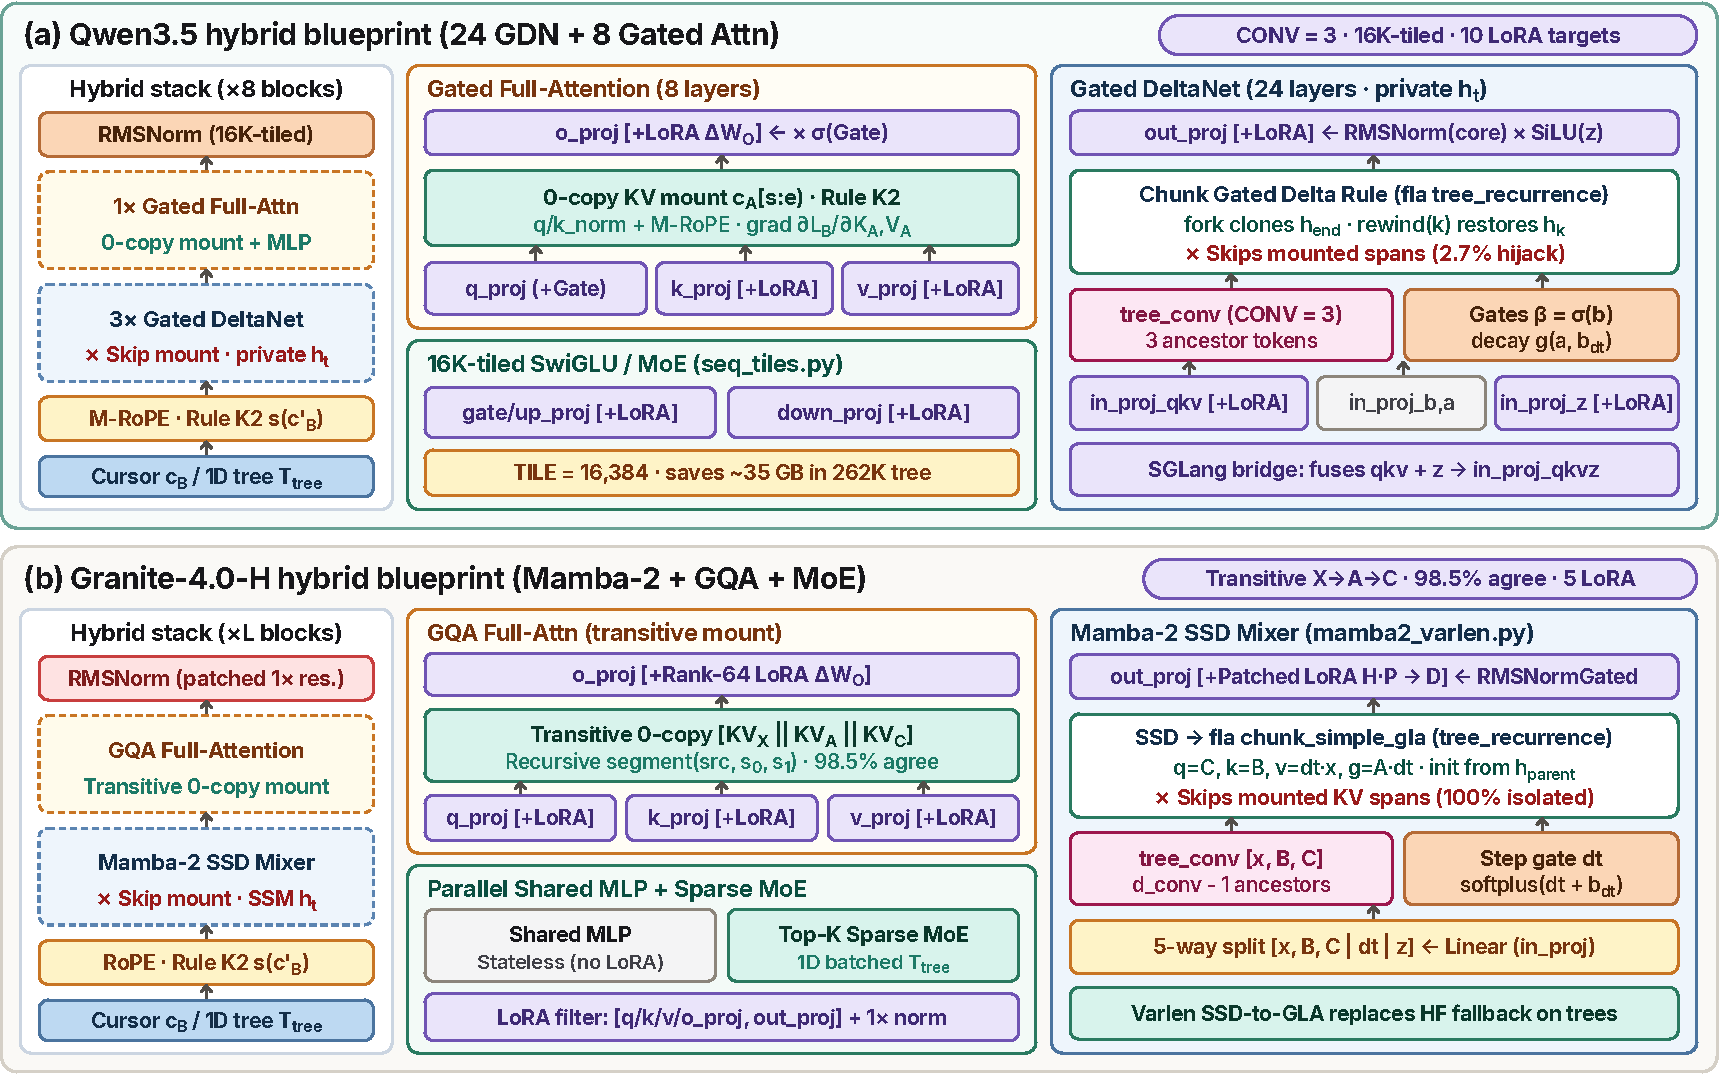
\includegraphics[width=1.0\textwidth]{figures/fig_arch_hybrid_gdn_mamba.pdf}
\captionsetup{type=figure, skip=5.5pt}
\captionof{figure}{Octopus integration blueprints for hybrid recurrent-attention models (\cref{tab:arch-hooks}). \textbf{(a) Qwen3.5 (Dense \& MoE Hybrid):} All $8$ Gated Attention layers 0-copy mount sibling KV pages $c_A[s:e)$, while $24$ GDN layers gather $\texttt{CONV\_CONTEXT}=3$ ancestor tokens (\texttt{tree\_conv}) and advance $\mathbf{h}_t$ along branch tokens via \texttt{fla}'s \texttt{chunk\_gated\_delta\_rule} (\texttt{tree\_recurrence}, skipping mounts $\to 2.7\%$ hijack), paired with $16\text{K}$ tiling (\texttt{seq\_tiles.py}) and fused \texttt{in\_proj\_qkvz} LoRA. \textbf{(b) Granite-4.0-H (Mamba-2 Hybrid):} Maps Mamba-2 SSD to \texttt{fla} \texttt{chunk\_simple\_gla}, supports transitive $X \leadsto A \leadsto C$ mounts ($98.5\%$ agree), and patches Mamba \texttt{out\_proj} LoRA and final RMSNorm.}
\label{fig:arch-hybrid}
\end{table}

\end{document}
